\documentclass[11pt,oneside]{article}
\usepackage[a4paper,margin=25mm,headheight=15pt]{geometry}
\usepackage[T1]{fontenc}
\usepackage[utf8]{inputenc}
\usepackage{libertinus}
\usepackage{amsmath,amssymb,amsthm,mathtools}
\usepackage{libertinust1math}
\usepackage{microtype,graphicx,booktabs,array,float}
\usepackage{xcolor}
\usepackage{enumitem}
\usepackage{fancyhdr}
\usepackage{hyperref}
\usepackage[nameinlink,noabbrev]{cleveref}
\hypersetup{colorlinks=true,linkcolor=blue!45!black,citecolor=blue!45!black,urlcolor=blue!45!black,
 pdftitle={Critical Complements in Fabius Conditioning},
 pdfauthor={Research draft prepared with ChatGPT for Vladimir Reshetnikov},
 pdfsubject={Sharp overlap, boundary information, and the order-zero Renyi crossover}}
\pagestyle{fancy}\fancyhf{}
\fancyhead[L]{\small Critical complements in Fabius conditioning}
\fancyhead[R]{\small Research article}
\fancyfoot[C]{\thepage}
\setlength{\parindent}{1.25em}
\setlength{\parskip}{3pt}
\setlength{\emergencystretch}{2em}
\numberwithin{equation}{section}
\theoremstyle{plain}
\newtheorem{theorem}{Theorem}[section]
\newtheorem{lemma}[theorem]{Lemma}
\newtheorem{proposition}[theorem]{Proposition}
\newtheorem{corollary}[theorem]{Corollary}
\theoremstyle{definition}
\newtheorem{definition}[theorem]{Definition}
\newtheorem{question}{Question}
\theoremstyle{remark}
\newtheorem{remark}[theorem]{Remark}
% ed. (2026-09-30): unnumbered environment for ProveIt editorial notes (the theorem counter is unchanged).
\newtheorem*{ednote}{Editorial note (ProveIt, 2026-09-30)}
% ed. (2026-10-01): a second unnumbered environment for the notes of 2026-10-01.
\newtheorem*{ednotelater}{Editorial note (ProveIt, 2026-10-01)}
\newcommand{\E}{\mathbb E}
\newcommand{\Pp}{\mathbb P}
\newcommand{\R}{\mathbb R}
\newcommand{\N}{\mathbb N}
\newcommand{\ind}{\mathbf 1}
\newcommand{\TV}{d_{\mathrm{TV}}}
\newcommand{\KL}{D_{\mathrm{KL}}}
\newcommand{\Law}{\mathcal L}
\newcommand{\OO}{\mathcal O}
\newcommand{\dd}{\,\mathrm d}
\newcommand{\Var}{\operatorname{Var}}
\newcommand{\Exp}{\operatorname{Exp}}
\newcommand{\Gam}{\operatorname{Gamma}}
\newcommand{\supp}{\operatorname{supp}}
\newcommand{\eps}{\varepsilon}
\newcommand{\repo}{\texttt{ProveIt}}
\newcommand{\sha}{\texttt{b8b0fa2184a044d46ce9ed0f25f88d7bb60fa042}}

\begin{document}
% ed. (2026-09-30): no page anchors on the title page, which is numbered 1 like the following page (removes a duplicate-destination warning of the delivered source).
\hypersetup{pageanchor=false}
\begin{titlepage}
\vspace*{12mm}
{\large\scshape Probability, asymptotic analysis, and information theory\par}
\vspace{12mm}
{\Huge\bfseries Critical Complements in\\[3mm] Fabius Conditioning\par}
\vspace{8mm}
{\Large Logarithmic overlap, finite-memory corrections,\\
and the order-zero R\'enyi crossover\par}
\vspace{14mm}
{\large Research draft prepared for Vladimir Reshetnikov\par}
{\normalsize Developed with ChatGPT\par}
\vspace{3mm}
{\large September 30, 2026\par}
\vspace{13mm}
\begin{abstract}
Exponential tilting turns a very small value of a geometric uniform
random series into a typical mean constraint. Previous work in the
\repo{} repository classifies the conditional law of a coordinate block
by its share of the tilted variance, but leaves the critical complement
regime as an explicit research question. We resolve the fixed-complement
case for geometric weights. After observing the active coordinates except
for a fixed number $r$ of early digits, the likelihood ratio reduces,
eventually exactly, to a density $h_r$ of a tilted boundary tail plus an
independent gamma variable. This gives the overlap expansion
\[
 1-\TV(P_{n,r},Q_{n,r})
 =\frac{\Lambda_n+r\log\Lambda_n+\log K-\log(r!)+1+o(1)}
 {\sqrt{2\pi n}},\qquad \Lambda_n=\tfrac12\log(2\pi n).
\]
A polynomial tail formula yields an all-orders inverse-logarithmic
expansion and an explicit residual endpoint defect. Every fixed positive
R\'enyi order has divergence $\Lambda_n$ minus the corresponding
boundary differential entropy, whereas order zero tends to $\log 2$.
We identify the intervening scale $\alpha\sqrt n=O(1)$ and its universal
normal-tail profile. With no early digit omitted, the remaining overlap
correction is positive and has logarithm asymptotic to
$-\sqrt{\log(1/q)\log n}$: the flat Fabius endpoint is visible in a
configuration-level information statistic. Proofs are self-contained;
228 exact algebra checks and reproducible numerical diagnostics accompany
the article.
\end{abstract}
\vfill
\noindent\small
\textbf{Status.} This is an unrefereed research manuscript with conventional
mathematical proofs, not a Lean-verified development. It resolves a precise
fixed-$r$ part of a repository research question, not every critical
complement regime. Worldwide priority and the description ``breakthrough''
are not certified. Classical tilting, gamma/simplex identities, and
small-deviation estimates are explicitly distinguished from the proposed
extensions.
\end{titlepage}
% ed. (2026-09-30): page anchors back on after the title page.
\hypersetup{pageanchor=true}

{\small\setlength{\parskip}{0pt}\tableofcontents}
\newpage

\section{The repository question and the contribution}
\label{sec:context}
The Fabius branch of \repo{} studies the compactly supported smooth
Fabius--Rvachev functions through exact values, Fourier products,
geometric uniform sums, and endpoint asymptotics. These connections are
also classical; see Arias de Reyna~\cite{arias,arithmetic}. The recent
repository manuscript \emph{Sharp Conditioning Laws for Uniform Random
Series}~\cite{repoSharp} develops a configuration-level theory rather
than only a scalar small-ball estimate.

That manuscript proves, for arbitrary positive summable weights, a
variance-fraction criterion for equivalence of a selected conditional
block and its exponentially tilted product marginal. At a fixed retained
variance fraction strictly below one it obtains Gaussian information
profiles. At fraction one it proves asymptotic separation. It also obtains
an independent exponential slack, a geometric boundary law, a bridge
limit, and the leading full-law overlap. We use this work to identify the
question, not as an unproved premise of the arguments below.

The source's question labelled \texttt{q:critical} asks what replaces the
Gaussian profile when the complement variance stays bounded, or diverges
much more slowly than the total variance. Its separate question
\texttt{q:edgeworth} concerns phase-sensitive higher corrections. The
fixed-complement case has two features that a Gaussian substitution cannot
recover: a genuinely non-Gaussian boundary density, and its very flat left
endpoint. This article makes both effects explicit.

\subsection{What is proved, and what is not}
Our retained block is $\{r+1,\ldots,n\}$ for a \emph{fixed} integer
$r\ge0$, along a fixed geometric phase. The omitted part contains $r$
strongly tilted early coordinates and the entire infinite geometric tail.
Its tilted variance tends to a positive finite constant, while the
retained variance is $n+O(1)$. We obtain a sharp overlap rate, its constant
and logarithmic corrections, an effective one-dimensional reduction,
all fixed positive information orders, and an order-zero transition.
The discarded coordinates and slack also admit an explicit joint
approximation in total variation with error $O((\log n)^2/n)$.

The case of a number $r=r_n$ tending to infinity is \emph{not} included in
these uniform error claims. Neither are arbitrary nongeometric weights,
several simultaneous constraints, an exact random-bit sampler, or a
machine-checked formalization. The last section formulates these as
further questions instead of treating them as corollaries.
% ed. (2026-09-30): an independent second answer to the same question was filed beside this package
\begin{ednote}
A second, independently written article under the same title,
\emph{Critical Complements in Fabius Conditioning: Sharp information loss,
geometric phase constants, and a logarithmic crossover}, is filed beside
this package as \path{../Critical_Complements_Sharp_Information_Loss/}
(batch~68 of the repository's \path{docs/incoming/}); neither article cites
the other. It answers the same question \texttt{q:critical} of
\cite{repoSharp} for different hidden coordinates: it observes the prefix
$\{1,\ldots,n-m\}$ and hides the last $m$ coordinates before the boundary
together with the tail, for every $m=o(n)$. For fixed $m$ it gives a
two-term overlap expansion with an explicit phase constant and relative
entropy to order $1/n$; for growing
$m$ it gives a leading overlap formula through the two real branches of
Lambert~$W$, with a change of regime at $m\asymp\log n$, and relative
entropy $\frac12\log(n/m)-\frac12+o(1)$. This article instead hides the
first $r$ coordinates together with the tail, for fixed $r$.
The two settings coincide only when nothing but the tail is hidden
($r=m=0$). That article's tilt is $t_n=\rho'q^{-(n+1)}$, so $\rho=\rho'/q$;
then its constant $K_{q,\rho',0}$ is $\log K$ of \eqref{eq:T}, its $R_0+E$
is $H_0$, its deficit $\Delta_0$ is $\delta_0$, and its corrected overlap
(its Theorem~2.1, \texttt{thm:fixed}, equation \texttt{eq:correctedtv}, at
$m=0$) is \cref{thm:flatmain}, proved independently. On filing, the value
$\log K=0.486134172\ldots$ of \eqref{eq:dyadicconstants} ($q=1/2$, $\rho=1$)
was reproduced from that article's formula for $K_{q,\rho',0}$ at
$\rho'=1/2$, and its tabulated $K_{1/2,1,0}=0.944809318$ equals $\log K$ at
$\rho=2$ (both to 30 digits). For $r\ge1$ or $m\ge1$ the two theorems
concern different marginals and do not conflict: the terms
$r\log\Lambda_n-\log(r!)$ here come from the $\Gam(r+1,1)$ part of $H_r$,
whereas the hidden coordinates there have a bounded sum. The words
``crossover'', $K$ (a product here, a logarithm there), $h$ (a density
here, an entropy there) and $\delta$ mean different things in the two
articles. The growing early-coordinate complement of the first question
of \cref{sec:future} is not treated there and remains open.
\end{ednote}
% ed. (2026-10-01): the logarithmic slice of that question is now treated (batch 71).
\begin{ednotelater}
Its logarithmic slice $r_n\asymp\log n$ is now treated, for the overlap
only, by a later article; see the note after that question in
\cref{sec:future}.
\end{ednotelater}

\subsection{Relation to existing methods}
Exponential-family conditioning and finite-block approximation have a
substantial history; Diaconis and Freedman~\cite{df} are an important
reference point. Small deviations of exponentially weighted independent
sums, including the leading logarithm-squared scale used below, belong to
an established theory~\cite{aurzada}. The information conventions are
standard~\cite{renyi}. The proposed contribution here is the particular
\emph{critical moving-block theorem package}: its exact boundary kernel,
sharp overlap expansion, inverse-logarithmic hierarchy, endpoint-defect
transfer, and order-zero crossover. The targeted source review does not
establish that no equivalent theorem exists elsewhere.

\section{Model, normalization, and the critical block}
\label{sec:model}
Fix $q\in(0,1)$ and $\rho>0$. All constants in asymptotic bounds may depend
on $q,\rho$, and a fixed $r$, unless otherwise stated. All logarithms are
natural. Under the original probability law $P$, let $(U_k)_{k\ge1}$ be
independent uniform variables on $[0,1]$, and define
\begin{equation}\label{eq:series}
 S_q=\sum_{k\ge1}q^kU_k,\qquad
 t_n=\rho q^{-n},\qquad Y_{n,k}=t_nq^kU_k.
\end{equation}
The series converges absolutely and is bounded by $q/(1-q)$. Write
\begin{equation}\label{eq:tilt}
 \frac{\dd Q_n}{\dd P}
   =\frac{e^{-t_nS_q}}{\E_P e^{-t_nS_q}},\qquad
 \mu_n=\E_{Q_n}(t_nS_q),\qquad x_n=\mu_n/t_n,
\end{equation}
and let $P_n=P(\,\cdot\mid S_q\le x_n)$. We condition the original law,
not $Q_n$, on the inequality. This distinction determines the slack
factor and all constants below.

Under $Q_n$ the variables $Y_{n,k}$ remain independent, and the variable
with cap $a_{n,k}=\rho q^{k-n}$ has density
\begin{equation}\label{eq:truncexp}
 e_a(y)=\frac{e^{-y}}{1-e^{-a}}\ind_{(0,a)}(y).
\end{equation}
Indeed, the tilt factors over every finite collection; the residual
bounded series supplies the independent remaining factor. Its mean and
variance, obtained by integrating or differentiating the normalizer, are
\begin{equation}\label{eq:mv}
 m(a)=1-\frac{a}{e^a-1},\qquad
 v(a)=1-\frac{a^2e^{-a}}{(1-e^{-a})^2}.
\end{equation}
As $a\downarrow0$, $m(a)=a/2+O(a^2)$ and $v(a)=a^2/12+O(a^4)$.
As $a\to\infty$, both tend to one exponentially fast.

\begin{definition}[Observed block and overlap]
For fixed $r\in\N\cup\{0\}$ and $n>r$, put
\[
 A_{n,r}=\{r+1,\ldots,n\},\qquad
 V_{n,r}=\sum_{k=r+1}^nY_{n,k},\qquad W_{n,r}=\mu_n-V_{n,r}.
\]
Let $P_{n,r}$ and $Q_{n,r}$ be the laws of the vector
$(Y_{n,k})_{k\in A_{n,r}}$ under $P_n$ and $Q_n$, respectively. Set
\begin{equation}\label{eq:overlapdef}
 \OO_{n,r}=1-\TV(P_{n,r},Q_{n,r}),\qquad
 c_n=(2\pi n)^{-1/2},\qquad \Lambda_n=-\log c_n.
\end{equation}
Here $\TV(P,Q)=\sup_B|P(B)-Q(B)|$, or one half of the $L^1$ distance
between densities. Thus $\OO=\int\min(p,q)$.
\end{definition}

We will reserve the letter $E_n$ for the \emph{actual slack}
$\mu_n-\sum_{k\ge1}Y_{n,k}$ under $P_n$. The observed deficit $W_{n,r}$
also includes the omitted contributions and is not the same variable.

\subsection{The Fabius specialization}
For $q=1/2$, $S_q$ is supported on $[0,1]$. Its distribution function
$F(x)=P(S_q\le x)$ obeys $S_q\overset d=(U+S_q')/2$, with independence.
Differentiating the resulting convolution gives
\[
 F'(x)=2\{F(2x)-F(2x-1)\},
\]
where $F=0$ to the left of zero and $F=1$ to the right of one. In
particular $F'(x)=2F(2x)$ for $0<x<1/2$. This is the probability
normalization of the Fabius function used in the geometric-sum
representation~\cite{arias}. Our event is therefore a Fabius endpoint
event when $q=1/2$, not an unrelated finite-dimensional surrogate.
% ed. (2026-09-30): Lean counterpart of the Fabius identification, not cited by the article
\begin{ednote}
This identification is machine-checked in the repository:
\path{Fabius.ProbabilityRepresentation.weightedSumCDF_eq_fabiusReal}
states that the distribution function of $\sum_{k\ge1}2^{-k}U_k$ is the
Fabius function on the whole real line, and
\path{Fabius.ProbabilityRepresentation.geometricUniformDensity_one_half_eq_rvachevUp}
gives its density as $2\,\mathrm{up}(2x-1)$; both are in
\path{Analysis/FabiusFunction/Lean/FabiusFunction/ProbabilityRepresentation.lean}.
No result of this article is formalized.
\end{ednote}

\section{The boundary kernel and the main results}
\label{sec:main}
Introduce an \emph{untilted} copy of the scaled geometric tail,
\begin{equation}\label{eq:T}
 T_\rho=\rho\sum_{j\ge1}q^jU_j,\qquad
 C=\frac{\rho q}{1-q},\qquad
 K=\frac1{\E e^{-T_\rho}}
   =\prod_{j\ge1}\frac{\rho q^j}{1-e^{-\rho q^j}}.
\end{equation}
Let $R_\rho$ have the exponentially tilted law of $T_\rho$:
\begin{equation}\label{eq:R}
 \Law(R_\rho)(\dd z)=K e^{-z}\Law(T_\rho)(\dd z).
\end{equation}
Equivalently, $R_\rho$ is a sum of independent variables of density
\eqref{eq:truncexp} with caps $\rho q^j$, $j\ge1$. It is exactly the
$Q_n$-law of $\sum_{k>n}Y_{n,k}$, for every $n$.

Let $G_{r+1}\sim\Gam(r+1,1)$ be independent of $R_\rho$. The
shape parameter is $r+1$, not $r$: the extra exponential is the
one-sided slack. Define
\begin{equation}\label{eq:Hr}
 H_r=R_\rho+G_{r+1},\qquad
 h_r(w)=\frac{K e^{-w}}{r!}\E (w-T_\rho)_+^r\quad(w>0).
\end{equation}
For $r=0$, $(w-T)_+^0$ in this formula means $\ind_{\{T<w\}}$;
thus $h_0(w)=K e^{-w}P(T_\rho<w)$. The value at an endpoint is immaterial.
We prove in \cref{sec:kernel} that $h_r$ is the probability density of
$H_r$.

\begin{theorem}[Sharp critical overlap]\label{thm:overlap}
For each fixed $q,\rho,r$ as above, as $n\to\infty$,
\begin{equation}\label{eq:mainoverlap}
 \OO_{n,r}=c_n\left\{
 \Lambda_n+r\log\Lambda_n+\log K-\log(r!)+1+o(1)\right\}.
\end{equation}
More precisely, with
\begin{equation}\label{eq:Jdef}
 J_r(z)=\int_0^\infty\min\{1,h_r(w)/z\}\dd w,
\end{equation}
one has the quantitative reduction
\begin{equation}\label{eq:quantJ}
 \frac{\OO_{n,r}}{c_n}=J_r(c_n)+O\!\left(\frac{(\log n)^3}{n}\right).
\end{equation}
The likelihood ratio of the full observed vector depends only on
$V_{n,r}$. Consequently all the divergences stated in this article are
also the divergences of the corresponding one-dimensional sum laws.
\end{theorem}

The leading coefficient of $\log n/\sqrt n$ is the same for every
fixed $r$. Omitting one additional early digit changes the next scale by
$\log\log n/\sqrt n$. The phase parameter enters already through
$\log K/\sqrt n$. Equal-prior optimal binary testing error is precisely
$\OO_{n,r}/2$, so the expansion has an immediate statistical meaning.

For a density $h$, write its differential R\'enyi entropies as
\begin{equation}\label{eq:entropydef}
 \mathfrak h_\alpha(h)=\frac{\log\int h^\alpha}{1-\alpha}
 \quad(0<\alpha<\infty,\ \alpha\ne1),\qquad
 \mathfrak h_1(h)=-\int h\log h,\qquad
 \mathfrak h_\infty(h)=-\log\|h\|_\infty.
\end{equation}
For probability measures, $D_\alpha(P\Vert Q)$ denotes the usual R\'enyi
divergence, with the continuous order-one and essential-supremum
order-infinity conventions~\cite{renyi}.

\begin{theorem}[Boundary information constants]\label{thm:entropy}
For every fixed $\alpha\in(0,\infty]$,
\begin{equation}\label{eq:renyifixed}
 D_\alpha(P_{n,r}\Vert Q_{n,r})
   =\Lambda_n-\mathfrak h_\alpha(h_r)+o(1).
\end{equation}
This includes
$\KL(P_{n,r}\Vert Q_{n,r})=\Lambda_n-\mathfrak h_1(h_r)+o(1)$.
Under $P_n$, $W_{n,r}$ converges to $H_r$ in total variation with error
$O((\log n)^2/n)$. The reverse relative entropy
$\KL(Q_{n,r}\Vert P_{n,r})$ is infinite for every sufficiently large $n$.
\end{theorem}

\begin{theorem}[The order-zero transition]\label{thm:crossover}
At order zero,
\begin{equation}\label{eq:orderzero}
 D_0(P_{n,r}\Vert Q_{n,r})\longrightarrow\log2.
\end{equation}
More generally, if $\alpha_n\ge0$ and $\alpha_n\sqrt n\to c\in[0,\infty)$,
then
\begin{equation}\label{eq:crossover}
 D_{\alpha_n}(P_{n,r}\Vert Q_{n,r})
 \longrightarrow
 \mathcal C(c):=-\log\!\left(e^{c^2/2}\Phi(-c)\right),
\end{equation}
where $\Phi$ is the standard normal distribution function. The limiting
function does not depend on $r,q$, or $\rho$.
\end{theorem}

\begin{theorem}[The flat-endpoint correction]\label{thm:flatmain}
Suppose $r=0$ and put $\lambda=\log(1/q)$. Define
\[
 \delta_0(z)=\int_0^C\left(1-\frac{h_0(w)}z\right)_+\dd w.
\]
For sufficiently large $n$,
\begin{equation}\label{eq:flatprecise}
 \frac{\OO_{n,0}}{c_n}
 =\Lambda_n+\log K+1-\delta_0(c_n)
      +O\!\left(\frac{(\log n)^3}{n}\right),
 \qquad
 \frac{\log\delta_0(c_n)}{\sqrt{\log n}}\longrightarrow-\sqrt\lambda.
\end{equation}
In particular the residual
\[
 \mathcal E_n=\Lambda_n+\log K+1-\frac{\OO_{n,0}}{c_n}
\]
is eventually strictly positive and satisfies
\begin{equation}\label{eq:flatresidual}
 \frac{\log\mathcal E_n}{\sqrt{\log n}}
   \longrightarrow-\sqrt{\log(1/q)}.
\end{equation}
\end{theorem}

This is a statement about the \emph{scaled} overlap residual. In the
unscaled overlap the correction is $c_n\delta_0(c_n)$. It is smaller
than $c_n(\log n)^{-M}$ for every fixed $M$, but larger than the
$O(c_n(\log n)^3/n)$ bulk error. No multiplicative equivalent for
$\delta_0$ is asserted.

\section{Exact boundary algebra and the variance clock}
\label{sec:kernel}
\begin{lemma}[Kernel formula and regularity]\label{lem:kernel}
The product $K$ in \eqref{eq:T} converges to a finite positive number,
and \eqref{eq:Hr} is a density. It is continuous, positive for $w>0$,
zero for $w\le0$, bounded by one, and has an exponentially decreasing
polynomial right tail. For every $\alpha>0$,
$\int h_r^\alpha<\infty$ and $\int|h_r\log h_r|<\infty$.
\end{lemma}
\begin{proof}
For small $a$, $\log(a/(1-e^{-a}))=a/2+O(a^2)$; summability of
$\rho q^j$ proves product convergence. The finite-coordinate Laplace
products tend to the infinite product by bounded convergence. Tilting
$T_\rho$ then gives \eqref{eq:R}; in particular
\[
 \E[e^{R_\rho}g(R_\rho)]=K\E[g(T_\rho)]
\]
for bounded measurable $g$. Convolve $R_\rho$ with the gamma density
$e^{-s}s^r/r!$ on $s>0$. The convolution equals
\[
 \frac{e^{-w}}{r!}\E\!\left[e^{R_\rho}(w-R_\rho)^r
                         \ind_{\{R_\rho<w\}}\right],
\]
which is \eqref{eq:Hr}. Hence its integral is one. The gamma density
is bounded by one (it is a convolution of $r+1$ rate-one exponential
densities), so the same is true after convolving with $R_\rho$.

The original tail $T_\rho$ has no atoms because its first uniform
summand has a density; it takes values arbitrarily near zero with
positive probability. This gives continuity and strict positivity of
$h_r$ on $(0,\infty)$, including the $r=0$ case. Since $T_\rho\le C$,
\eqref{eq:Hr} is bounded for large $w$ by a constant times
$e^{-w}(1+w)^r$. Every positive power is therefore integrable. Finally
$y|\log y|\le C_0\sqrt y$ on $0<y\le1$, which proves the entropy
integrability assertion.
\end{proof}

Let $m_j^*=\E T_\rho^j$, with $m_0^*=1$, and define the monic polynomial
\begin{equation}\label{eq:polynomial}
 p_r(w)=\E(w-T_\rho)^r
       =\sum_{j=0}^r(-1)^j\binom rj m_j^*w^{r-j}.
\end{equation}
Then for $w\ge C$,
\begin{equation}\label{eq:tailpoly}
 h_r(w)=\frac K{r!}e^{-w}p_r(w),\qquad
 p_r'(w)=r p_{r-1}(w).
\end{equation}
The entire infinite boundary enters this tail through finitely many
ordinary moments and the scalar $K$. It is important that these are the
moments of \emph{untilted} $T_\rho$, not of $R_\rho$.

\begin{proposition}[Exact moment recursion]\label{prop:moments}
The moments satisfy
\begin{equation}\label{eq:momentrec}
 m_k^*=
 \frac1{1-q^k}\sum_{j=0}^{k-1}
 \binom kj\frac{(\rho q)^{k-j}q^j}{k-j+1}\,m_j^*,\qquad k\ge1.
\end{equation}
Thus $m_k^*$ is rational whenever $q$ and $\rho$ are rational. The
kernels also satisfy
\begin{equation}\label{eq:kernelrec}
 \left(\frac{\dd}{\dd w}+1\right)h_{r+1}(w)=h_r(w),\qquad w>0.
\end{equation}
\end{proposition}
\begin{proof}
The identity $T_\rho\overset d=\rho qU+qT_\rho'$ has independent terms.
Taking its $k$th moment, the term $j=k$ on the right is $q^km_k^*$;
isolating it gives \eqref{eq:momentrec}. The uniform moment is
$\E U^{k-j}=1/(k-j+1)$. Differentiating the integrated positive-part
formula in \eqref{eq:Hr} proves \eqref{eq:kernelrec}; for $r=0$ this
uses the continuous distribution function of $T_\rho$. Equivalently,
$h_{r+1}=h_r*e^{-w}\ind_{w>0}$, which gives the same identity.
\end{proof}

\begin{proposition}[Mean, variance, and phase dependence]\label{prop:clock}
Write $\mu_R=\E R_\rho$ and $\sigma_R^2=\Var R_\rho$. Then
\begin{align}
 \mu_n&=n+\kappa+o(1),&
 \kappa&=\mu_R-\sum_{j\ge0}\frac{\rho q^{-j}}{e^{\rho q^{-j}}-1},
 \label{eq:kappa}\\
 \Var_{Q_n}\!\left(\sum_{k\ge1}Y_{n,k}\right)&=n+\nu+o(1),&
 \nu&=\sigma_R^2-\sum_{j\ge0}\{1-v(\rho q^{-j})\}.
 \label{eq:nu}
\end{align}
For fixed $r$ the omitted variance is $r+\sigma_R^2+o(1)$, and
\begin{equation}\label{eq:criticalfraction}
 \frac{\Var_{Q_n}V_{n,r}}
 {\Var_{Q_n}(\sum_{k\ge1}Y_{n,k})}
 =1-\frac{r+\sigma_R^2}{n}+o(n^{-1}).
\end{equation}
Furthermore
\begin{equation}\label{eq:phaseK}
 \frac{\dd}{\dd\rho}\log K=\frac{\mu_R}{\rho}>0.
\end{equation}
\end{proposition}
\begin{proof}
Reindex the first $n$ caps as $\rho q^{-j}$, $0\le j<n$. Their
mean sum is $n-\sum_{j=0}^{n-1}(1-m(\rho q^{-j}))$; the remaining
mean is $\mu_R$. The deficits decrease superexponentially in $j$, so
the sum converges and its omitted part tends to zero. Apply the same
argument to variances. The first $r$ caps tend to infinity, so their
variances tend to one. Independence gives \eqref{eq:criticalfraction}.
Finally differentiate the convergent product locally uniformly in
$\rho>0$. The derivative of its $j$th logarithm is
$m(\rho q^j)/\rho$; summing proves \eqref{eq:phaseK}.
\end{proof}

One may restrict $\rho$ to $[1,q^{-1})$ to use a canonical multiplicative
phase. None of the proofs needs that restriction. No uniformity as
$q\to1$, $\rho\to0$, or $r\to\infty$ is implicit.

\section{An eventually exact likelihood-ratio formula}
\label{sec:likelihood}
Let $f_{n,r}$ be the density of $V_{n,r}$ under $Q_n$, extended by zero
outside its support. The next identity is the reason the problem remains
tractable even though the retained vector has growing dimension.

\begin{theorem}[Exact critical kernel]\label{thm:exact}
For every sufficiently large $n$, define
\begin{equation}\label{eq:Z}
 Z_{n,r}=\int_0^\infty f_{n,r}(\mu_n-w)h_r(w)\dd w.
\end{equation}
Then
\begin{equation}\label{eq:likelihood}
 \frac{\dd P_{n,r}}{\dd Q_{n,r}}(y)
   =\frac{h_r(\mu_n-\sum_{k\in A_{n,r}}y_k)}{Z_{n,r}}.
\end{equation}
Under $P_n$, the density of the observed deficit $W_{n,r}$ is
\begin{equation}\label{eq:deficitdensity}
 g_{n,r}(w)=\frac{f_{n,r}(\mu_n-w)h_r(w)}{Z_{n,r}}.
\end{equation}
\end{theorem}
\begin{proof}
Set $B_n=\E_{Q_n}[e^{T_n-\mu_n}\ind_{\{T_n\le\mu_n\}}]$, where
$T_n=\sum_{k\ge1}Y_{n,k}$. Undoing the tilt in \eqref{eq:tilt} gives
\[
 \frac{\dd P_n}{\dd Q_n}
 =\frac{e^{T_n-\mu_n}\ind_{\{T_n\le\mu_n\}}}{B_n}.
\]
Split $T_n=V_{n,r}+L_n^{\mathrm{lost}}$, with the two parts independent
under $Q_n$. Integrating out the lost part, and writing
$w=\mu_n-v$, gives the marginal numerator
\begin{equation}\label{eq:rawkernel}
 e^{-w}\E_{Q_n}\!
   [e^{L_n^{\mathrm{lost}}}\ind_{\{L_n^{\mathrm{lost}}\le w\}}].
\end{equation}
This is the density at $w$ of $L_n^{\mathrm{lost}}+E$, where
$E\sim\Exp(1)$ is independent.

The lost part consists of the first $r$ coordinates and a tail with
law $R_\rho$. If $r>0$, its smallest early cap is
$a_{n,r}=\rho q^{r-n}$, and $\mu_n<a_{n,r}$ eventually by
\cref{prop:clock}. On the domain in \eqref{eq:rawkernel}, where
$0\le w\le\mu_n$, every early lost coordinate is below every early
cap. Their joint density is therefore the joint density of $r$
independent rate-one exponentials multiplied by the constant
\[
 p_{n,r}^{-1},\qquad
 p_{n,r}=\prod_{k=1}^r(1-e^{-a_{n,k}}).
\]
For $r=0$, set $p_{n,0}=1$. Thus \eqref{eq:rawkernel} equals
$h_r(w)/p_{n,r}$ throughout the only region accessible to the
nonnegative observed sum. The same constant occurs in $B_n$, so it
cancels. In fact $Z_{n,r}=p_{n,r}B_n$. This proves
\eqref{eq:likelihood}; changing variables from $v$ to $w$ proves
\eqref{eq:deficitdensity}.
\end{proof}

\begin{remark}[Which normalizer is being used]
$Z_{n,r}$ is the normalizer for the fixed limiting kernel $h_r$.
For $r>0$ it is not literally the original rejection normalizer $B_n$,
although $p_{n,r}\to1$ extremely fast. Keeping the exact factor
$p_{n,r}$ prevents a finite-$n$ normalization error.
\end{remark}

\begin{corollary}[Sufficiency of the sum]\label{cor:sufficiency}
Every integral divergence obtained by integrating a function of
$\dd P_{n,r}/\dd Q_{n,r}$ is unchanged when the observed vector is
replaced by its sum $V_{n,r}$. This includes overlap, total variation,
relative entropy, and every R\'enyi order used here.
\end{corollary}
\begin{proof}
The likelihood ratio in \eqref{eq:likelihood} is a measurable function
of the sum. The pushforward likelihood ratio is the same function,
since integration over each sum preimage leaves it unchanged. The two
integrals are then equal by the definition of pushforward measure.
The essential supremum is likewise unchanged.
\end{proof}

\section{A local density estimate with an elementary proof}
\label{sec:local}
We need a local approximation on a logarithmic window, not a central
limit theorem alone. In this geometric setting it can be proved directly
from a large gamma core and a small boundary block.

\begin{lemma}[Gamma-core local estimate]\label{lem:local}
For fixed $q,\rho,r$, there is a constant $C_0$ such that
\begin{equation}\label{eq:globalsup}
 \sup_v f_{n,r}(v)\le C_0 n^{-1/2}
\end{equation}
for sufficiently large $n$. For every fixed $B>0$,
\begin{equation}\label{eq:localdensity}
 \sup_{|u|\le B\log n}
 \left|\frac{f_{n,r}(\E_{Q_n}V_{n,r}+u)}{c_n}-1\right|
   =O_B\!\left(\frac{(\log n)^2}{n}\right).
\end{equation}
Also
\begin{equation}\label{eq:CLT}
 \frac{V_{n,r}-\E_{Q_n}V_{n,r}}{\sqrt n}
   \ \Rightarrow\ N(0,1).
\end{equation}
\end{lemma}
\begin{proof}
Choose a large fixed $M$, say $M>10$. Take
$\ell_n=O(\log\log n)$ so that the smallest cap in the core
$\{r+1,\ldots,n-\ell_n\}$ is at least $M\log n$; the remaining
$\ell_n$ coordinates form a boundary block. Denote the core size by
$N=n-r-\ell_n$.

\emph{Step 1: removing core caps.}
The core law is exactly a vector of $N$ independent exponentials
conditioned to stay below its coordinate caps. If the smallest cap is
$a$, a union bound bounds the probability of a violation by
\[
 \sum_{j\ge0}e^{-a q^{-j}}
 \le\frac{e^{-a}}{1-e^{-a(q^{-1}-1)}}=O(n^{-M}).
\]
Here $q^{-j}\ge1+j(q^{-1}-1)$. Hence the actual core sum and a
$\Gam(N,1)$ sum differ in total variation by $O(n^{-M})$. Their means
differ by at most
$\sum a_j/(e^{a_j}-1)=O((\log n)n^{-M})$.

Let $D_n$ be the sum of the boundary block, independent of either
core construction. It contains the last coordinate, whose density is
bounded by $(1-e^{-\rho})^{-1}$. Consequently its density has the same
upper bound. Convolution upgrades the total-variation error of the
core to a uniform density error $O(n^{-M})$ for the full sum: for
measures $\eta,\eta'$ and a bounded density $d$,
\[
 \sup_x|((\eta-\eta')*d)(x)|
 \le 2\|d\|_\infty\TV(\eta,\eta').
\]
Thus it suffices to analyze $G_N+D_n$, where $G_N\sim\Gam(N,1)$.

\emph{Step 2: size of the boundary block.}
A capped exponential is stochastically dominated by an uncapped
rate-one exponential. This follows, for example, by coupling their
inverse distribution functions:
\[
 -\log\{1-(1-e^{-a})U\}\le-\log(1-U).
\]
Therefore $\E D_n\le\ell_n$ and
$\E e^{D_n/2}\le2^{\ell_n}$. For every prescribed $A>0$, choosing a
fixed sufficiently large $M'$ gives
\begin{equation}\label{eq:Dbound}
 P(D_n>M'\log n)\le2^{\ell_n}n^{-M'/2}=O(n^{-A}).
\end{equation}

\emph{Step 3: the gamma density near its mean.}
Write $\gamma_N(x)=e^{-x}x^{N-1}/\Gamma(N)$ for $x>0$.
Stirling's formula with its $O(N^{-1})$ logarithmic remainder,
followed by the Taylor expansion of $\log(1+s/N)$, gives
\begin{equation}\label{eq:gammalocal}
 \gamma_N(N+s)=\frac1{\sqrt{2\pi N}}
   \left\{1+O\!\left(\frac{1+s^2}{N}\right)\right\}
 \quad\text{uniformly for }|s|\le C\log n.
\end{equation}
For clarity, the logarithm of the density minus
$-\tfrac12\log(2\pi N)$ is
$-s/N-s^2/(2N)+O(N^{-1}+s^2/N^2+|s|^3/N^2)$ on this window.
This tends to zero uniformly and implies \eqref{eq:gammalocal}.
The gamma density has its maximum at $N-1$ when $N>1$, so Stirling
also gives $\|\gamma_N\|_\infty\le C_1/\sqrt N$.

At $v=\E V_{n,r}+u$ with $|u|\le B\log n$, the argument
$v-D_n$ is $N+O(\log n)$ on the event in \eqref{eq:Dbound}.
Integrate \eqref{eq:gammalocal} over that event. Its complement is
bounded using the global gamma maximum and \eqref{eq:Dbound}.
Replacing $N$ by $n$ changes the leading density by
$1+O(\log\log n/n)$, within the stated error. The uniform
$O(n^{-M})$ density error from Step 1 is smaller still after division
by $c_n$. This proves \eqref{eq:localdensity}; the global maximum
bound and the convolution error prove \eqref{eq:globalsup}.

\emph{Step 4: the central limit theorem.}
The centered gamma core is the sum of $N$ centered independent
exponentials. Its characteristic function at $u/\sqrt N$ is
\[
 \left(\frac{e^{-iu/\sqrt N}}{1-iu/\sqrt N}\right)^N
 \longrightarrow e^{-u^2/2},
\]
by expanding the logarithm. Hence it converges to the standard
normal law. The centered boundary block divided by $\sqrt n$
tends to zero in probability, since
$\E|D_n-\E D_n|\le2\ell_n=o(\sqrt n)$.
The core total-variation error tends to zero and $N/n\to1$.
These facts yield \eqref{eq:CLT}.
\end{proof}

\begin{corollary}[Normalizer and local flatness at the constraint]
\label{cor:normalizer}
For fixed $B>0$,
\begin{align}
 Z_{n,r}&=c_n\{1+O((\log n)^2/n)\},\label{eq:Zasymp}\\
 \frac{f_{n,r}(\mu_n-w)}{c_n}
   &=1+O_B((\log n)^2/n),\qquad 0\le w\le B\log n.
 \label{eq:flatbulk}
\end{align}
Moreover $f_{n,r}(\mu_n-w)/c_n$ is bounded uniformly in $w,n$.
\end{corollary}
\begin{proof}
The difference $\mu_n-\E V_{n,r}$ is the omitted mean, which tends
to $r+\mu_R$ and is bounded. Thus \eqref{eq:flatbulk} follows from
\cref{lem:local}. Integrate it against $h_r$ on $[0,B\log n]$.
The omitted tail has mass $O(n^{-B}(\log n)^r)$ by
\eqref{eq:tailpoly}; the global bound controls its contribution.
Taking $B$ sufficiently large proves \eqref{eq:Zasymp}.
\end{proof}

\begin{corollary}[A joint critical-complement approximation]
\label{cor:joint}
Under $P_n$, the joint law of the first $r$ rescaled digits, the
entire rescaled tail after $n$, and the actual slack $E_n$ is within
$O((\log n)^2/n)$ in total variation of
\begin{equation}\label{eq:jointproduct}
 \Exp(1)^{\otimes r}\ \otimes\
 \bigotimes_{j\ge1} e_{\rho q^j}(z_j)\dd z_j\ \otimes\ \Exp(1).
\end{equation}
In particular $W_{n,r}$ is within the same order of total variation
of $H_r$.
\end{corollary}
\begin{proof}
The exact cancellation in \cref{thm:exact}, now retaining all lost
coordinates and the slack, gives the joint likelihood ratio
\[
 \frac{f_{n,r}(\mu_n-w)}{Z_{n,r}},\qquad
 w=\sum_{i=1}^r e_i+\sum_{j\ge1}z_j+e,
\]
relative to the product law in \eqref{eq:jointproduct}. This can also
be checked directly: transforming the observed sum to the slack
multiplies its density by $e^{-e}$ after undoing the tilt; the early
lost coordinate densities are constant multiples of $e^{-e_i}$,
and those constants cancel the normalizer as before. Under the
product reference, $w$ has density $h_r$.

On $w\le B\log n$, \cref{cor:normalizer} bounds the likelihood ratio
minus one by $O((\log n)^2/n)$. On the complement the ratio is
uniformly bounded, and the reference mass is
$O(n^{-B}(\log n)^r)$. Integrating the absolute difference proves
the assertion. Taking the sum is a measurable map and cannot
increase total variation.
\end{proof}

The qualitative independence of boundary coordinates and slack is
already part of the preceding repository work. The quantitative
fixed-complement estimate above is included to make the later
information limits independent of any unproved uniform local theorem.

\section{Overlap: a logarithmic threshold and an exact tail formula}
\label{sec:overlap}
\subsection{Reduction to a fixed density}
\begin{proof}[Proof of \eqref{eq:quantJ}]
By \cref{thm:exact},
\begin{equation}\label{eq:overlapintegral}
 \OO_{n,r}=\int_0^\infty f_{n,r}(\mu_n-w)
                 \min\{1,h_r(w)/Z_{n,r}\}\dd w.
\end{equation}
Put $\eps_n=(\log n)^2/n$ and choose a sufficiently large fixed
$B$. On $[0,B\log n]$, replacing $f_{n,r}/c_n$ by one introduces
an error $O(\eps_n\log n)$. Replacing $Z_{n,r}$ by $c_n$ has the
same cost: if $Z/c=1+O(\eps_n)$, then for every $h\ge0$,
\[
 |\min(1,h/Z)-\min(1,h/c)|
 \le C_2\eps_n\min(1,h/c).
\]
The integral of the last minimum is $O(\log n)$, since it is at
most $B\log n$ on the window, and at most
$c_n^{-1}\int_{B\log n}^\infty h_r$ outside it. The tails in
\eqref{eq:overlapintegral}, after division by $c_n$, have this same
upper bound times a fixed constant. They are
$O(n^{1/2-B}(\log n)^r)$, negligible compared with
$(\log n)^3/n$ when $B$ is chosen large. This proves the reduction.
\end{proof}

\subsection{A finite polynomial controls the upper threshold}
Put $A=K/r!$, and choose the fixed cutoff $D=C+r+1$. The symbol $D$
in this subsection is a cutoff, not a divergence. For sufficiently
small $z>0$, let $b_r(z)>D$ be the unique solution of
\begin{equation}\label{eq:upperroot}
 A e^{-b_r(z)}p_r(b_r(z))=z,
\end{equation}
and define the left endpoint defect
\begin{equation}\label{eq:deltar}
 \delta_r(z)=\int_0^D\left(1-\frac{h_r(w)}z\right)_+\dd w.
\end{equation}
The value of this integral is unchanged by enlarging the fixed cutoff
once $z$ is sufficiently small.

\begin{proposition}[Exact decomposition of the overlap kernel]
\label{prop:Jexact}
For all sufficiently small $z>0$,
\begin{equation}\label{eq:Jexact}
 J_r(z)=b_r(z)+
 \frac{\displaystyle\sum_{j=0}^r p_r^{(j)}(b_r(z))}{p_r(b_r(z))}
 -\delta_r(z).
\end{equation}
In particular $\delta_r(z)\to0$ as $z\downarrow0$.
\end{proposition}
\begin{proof}
For $w>C$,
\[
 \frac{p_r'(w)}{p_r(w)}
 =\frac{r\E(w-T_\rho)^{r-1}}{\E(w-T_\rho)^r}
 \le\frac r{w-C},
\]
with zero numerator when $r=0$. Thus $e^{-w}p_r(w)$ is strictly
decreasing on $[D,\infty)$ and tends to zero. If $z<h_r(D)$,
the root \eqref{eq:upperroot} exists and is unique. Repeated integration
by parts, which terminates after $r$ steps, gives
\[
 \int_b^\infty e^{-w}p_r(w)\dd w
   =e^{-b}\sum_{j=0}^r p_r^{(j)}(b).
\]
The integral defining $J_r$ is $D-\delta_r(z)$ on $[0,D]$,
is $b_r(z)-D$ on $[D,b_r(z)]$, and is the displayed tail integral
multiplied by $A/z$ thereafter. Equation \eqref{eq:upperroot}
cancels the last exponential and proves \eqref{eq:Jexact}.
Finally $h_r(w)>0$ for every $w>0$, so dominated convergence on
$[0,D]$ gives $\delta_r(z)\to0$.
\end{proof}

\begin{proof}[Proof of \cref{thm:overlap}]
Set $z=c_n$ and abbreviate $b=b_r(c_n)$, $\Lambda=\Lambda_n$.
Taking logarithms in \eqref{eq:upperroot}, and using
$p_r(b)=b^r(1+O(b^{-1}))$, gives
\[
 b=\Lambda+\log A+r\log b+O(b^{-1}).
\]
First this implies $b/\Lambda\to1$; substituting back then gives
$b=\Lambda+r\log\Lambda+\log A+o(1)$. The rational tail factor
in \eqref{eq:Jexact} tends to one, and $\delta_r(c_n)\to0$.
Combine with \eqref{eq:quantJ} and $\log A=\log K-\log(r!)$.
The sufficiency assertion follows from \cref{cor:sufficiency}.
\end{proof}

\subsection{The inverse-logarithmic hierarchy}
The exact decomposition is stronger than the three-term formula.
For the next statement put
\[m_1^*=\frac{\rho q}{2(1-q)},\qquad d_n=r\log\Lambda_n+\log A.\]

\begin{proposition}[First higher correction and all orders]
\label{prop:allorders}
For fixed $r$, one has
\begin{align}
 \frac{\OO_{n,r}}{c_n}
 ={}&\Lambda_n+d_n+1
 +\frac{r d_n+r(1-m_1^*)}{\Lambda_n}-\delta_r(c_n) \nonumber\\
 &+O\!\left(\frac{(\log\Lambda_n)^2}{\Lambda_n^2}
               +\frac{(\log n)^3}{n}\right).
 \label{eq:firsthigher}
\end{align}
More generally, for every fixed integer $M\ge1$ there are explicitly
recursive polynomials $A_1(X),\ldots,A_M(X)$, with
$\deg A_j\le j$, such that
\begin{align}
 \frac{\OO_{n,r}}{c_n}
 ={}&\Lambda_n+r\log\Lambda_n+\log A+1
       +\sum_{j=1}^M\frac{A_j(\log\Lambda_n)}{\Lambda_n^j}
       -\delta_r(c_n) \nonumber\\
 &+O\!\left(\frac{(\log\Lambda_n)^{M+1}}{\Lambda_n^{M+1}}
               +\frac{(\log n)^3}{n}\right).
 \label{eq:allorders}
\end{align}
Their coefficients depend only on $r,K,m_1^*,\ldots,m_r^*$.
In particular
$A_1(X)=r^2X+r\log A+r(1-m_1^*)$.
For $r=0$, all these polynomials vanish and the upper-tail part of
\eqref{eq:Jexact} is exactly $\Lambda_n+\log K+1$.
\end{proposition}
\begin{proof}
For large $b$,
\[
 \log p_r(b)=r\log b-\frac{r m_1^*}{b}+O(b^{-2}).
\]
Writing $b=\Lambda+d+\eta$ in the logarithmic root equation and
expanding $\log b$ yields
\[
 b=\Lambda+d+\frac{rd-rm_1^*}{\Lambda}
      +O((\log\Lambda)^2/\Lambda^2).
\]
The rational tail factor in \eqref{eq:Jexact} is
$1+r/b+O(b^{-2})$. Combining these proves \eqref{eq:firsthigher}.

For completeness the same procedure has controlled remainders at
every fixed order. Write
$p_r(b)=b^r(1+a_1/b+\cdots+a_r/b^r)$ and consider
\[
 F(b)=b-r\log b-\log(1+a_1/b+\cdots+a_r/b^r).
\]
For sufficiently large $b$, $F'(b)=1-r/b+O(b^{-2})>1/2$.
Starting with $b_0=\Lambda+r\log\Lambda+\log A$, substitute
\[
 b_M=b_0+\sum_{j=1}^M B_j(\log\Lambda)\Lambda^{-j}
\]
into $F(b_M)=\Lambda+\log A$. Taylor-expand the logarithms in
$\Lambda^{-1}$. At order $\Lambda^{-j}$ the new polynomial $B_j$
appears with coefficient one; all other terms are already determined.
Set $B_j$ equal to their negative. Products of the previous terms
show inductively that $\deg B_j\le j$. Taylor's theorem gives a
residual $O((\log\Lambda)^{M+1}/\Lambda^{M+1})$. Since $F'>1/2$,
the mean value theorem bounds $|b-b_M|$ by twice this residual.

The rational function $\sum p_r^{(j)}/p_r$ has a convergent power
series in $1/b$ near infinity. Substitute the same $b_M$ and expand
to order $M$; its bounded derivative transfers the root remainder.
This gives the polynomials $A_j$ and the stated error for $J_r$.
Equation \eqref{eq:quantJ} adds the bulk error. When $r=0$,
$p_0=1$, $b=\Lambda+\log K$, and the tail factor is exactly one.
\end{proof}

Section~\ref{sec:flat} proves that $\delta_r(c_n)$ is smaller than every
fixed inverse power of $\Lambda_n$. Thus \eqref{eq:allorders} is also
an ordinary all-orders inverse-logarithmic expansion after suppressing
the defect. Retaining the defect is substantially more informative at
accessible values of $n$, and is essential when $r=0$.

\section{Information constants and the non-Gaussian deficit}
\label{sec:information}
\begin{proof}[Proof of \cref{thm:entropy}]
The total-variation statement is \cref{cor:joint}. For
$0<\alpha<\infty$, $\alpha\ne1$, the exact likelihood formula gives
\begin{equation}\label{eq:renyiintegral}
 \exp\{(\alpha-1)D_\alpha(P_{n,r}\Vert Q_{n,r})\}
 =Z_{n,r}^{-\alpha}\int_0^\infty
          f_{n,r}(\mu_n-w)h_r(w)^\alpha\dd w.
\end{equation}
For every fixed $w>0$, $f_{n,r}(\mu_n-w)/c_n\to1$, and the ratio
is uniformly bounded by \cref{cor:normalizer}. Since $h_r^\alpha$
is integrable, dominated convergence implies
\[
 \int_0^\infty f_{n,r}(\mu_n-w)h_r(w)^\alpha\dd w
   =c_n\left\{\int_0^\infty h_r(w)^\alpha\dd w+o(1)\right\}.
\]
Combine this with $Z_{n,r}/c_n\to1$ in \eqref{eq:renyiintegral}.
Taking the logarithm and dividing by $\alpha-1$ proves
\eqref{eq:renyifixed} for these orders.

For order one, \eqref{eq:deficitdensity} gives the exact identity
\begin{equation}\label{eq:KLexact}
 \KL(P_{n,r}\Vert Q_{n,r})
 =-\log Z_{n,r}
 +\frac1{Z_{n,r}}\int_0^\infty
       f_{n,r}(\mu_n-w)h_r(w)\log h_r(w)\dd w.
\end{equation}
The same argument now uses the integrability of $|h_r\log h_r|$
from \cref{lem:kernel}. This proves the Shannon-entropy constant.

The continuous density $h_r$ tends to zero at zero and infinity, so
it attains a positive maximum at some finite $w>0$. For large $n$,
this point lies in the interior of the accessible range of
$\mu_n-V_{n,r}$. Indeed $\mu_n\sim n$, whereas the observed sum's
support has an exponentially large upper endpoint. The density
$f_{n,r}$ is strictly positive in its support interior. Consequently
the essential supremum of the likelihood ratio is exactly
$\|h_r\|_\infty/Z_{n,r}$, proving the order-infinity formula.

Finally $P_{n,r}(V_{n,r}>\mu_n)=0$, whereas the same event has
positive $Q_{n,r}$ probability for large $n$ (in fact tending to
one half by \eqref{eq:CLT}). Thus $Q_{n,r}$ is not absolutely
continuous with respect to $P_{n,r}$, and the reverse relative
entropy is infinite.
\end{proof}

\begin{remark}[Rates for fixed information orders]
The proof also gives an $O_\alpha((\log n)^2/n)$ remainder in
\eqref{eq:renyifixed} for each \emph{fixed} positive order, including
one and infinity. To see this, use \eqref{eq:flatbulk} on
$[0,B\log n]$ and the exponential-polynomial tail of $h_r^\alpha$
outside it, choosing $B$ large depending on $\alpha$. For order one
use $h_r|\log h_r|$ instead. The positive integral
$\int h_r^\alpha$ is fixed, so taking its logarithm preserves the
error order. The resulting constants are not uniform as
$\alpha\downarrow0$. The theorem in the next section shows why
such a qualification is essential.
\end{remark}

\subsection{Hellinger affinity and the meaning of the constant}
The Hellinger affinity has the particularly transparent form
\begin{equation}\label{eq:affinity}
 \int\sqrt{\dd P_{n,r}\dd Q_{n,r}}
 =(2\pi n)^{-1/4}\int_0^\infty\sqrt{h_r(w)}\dd w\,(1+o(1))
 =(2\pi n)^{-1/4}e^{\mathfrak h_{1/2}(h_r)/2}(1+o(1)).
\end{equation}
This follows either directly from \eqref{eq:renyiintegral} or by
setting $\alpha=1/2$ in \cref{thm:entropy}.

The retained vector is high-dimensional, but its conditional likelihood
is concentrated in an $O(1)$ deficit window, whose profile is $h_r$.
The canonical sum density is approximately $c_n$ on that window.
The factor $-\log c_n=\Lambda_n$ therefore measures the
large-scale concentration cost, while $\mathfrak h_\alpha(h_r)$
measures the remaining microscopic spread. The overlap samples a
larger window, of width $\Lambda_n+r\log\Lambda_n+O(1)$, because its
integrand is clipped at one. This distinction explains why the overlap
contains a logarithmic factor that is absent from the affinity.

All fixed nonnegative moments of $W_{n,r}$ also converge to those of
$H_r$. For any fixed moment order the error is $O((\log n)^2/n)$:
multiply the argument in \cref{cor:joint} by $w^k$, use the uniform
likelihood bound, and choose a sufficiently large logarithmic cutoff.
This moment statement is separate from entropy convergence, which
required the logarithmic integrability check above.

\section{A universal transition at R\'enyi order zero}
\label{sec:crossover}
At order zero the divergence records only the $Q$-mass of the
support of $P$. A narrow high-density region can have a large
positive-order divergence while still having a support of macroscopic
$Q$-mass. This distinction is realized sharply here.

\begin{proof}[Proof of \cref{thm:crossover}]
Since $h_r(w)>0$ exactly for $w>0$, the support-mass formula is
\begin{equation}\label{eq:D0exact}
 D_0(P_{n,r}\Vert Q_{n,r})
   =-\log Q_n(V_{n,r}<\mu_n).
\end{equation}
By \cref{lem:local} and the bounded difference
$\mu_n-\E V_{n,r}$, the standardized deficit $W_{n,r}/\sqrt n$
converges under $Q_n$ to the standard normal law. This proves
\eqref{eq:orderzero}.

Now let $\alpha_n>0$ with $\alpha_n\sqrt n\to c<\infty$; zero
orders occurring along a subsequence are already covered. For fixed
$0<\eta<M<\infty$, the polynomial tail formula implies uniformly
for $z\in[\eta,M]$,
\begin{equation}\label{eq:tailvaryingorder}
 \log h_r(\sqrt n z)
 =-\sqrt n z+r\log(\sqrt n z)+\log(K/r!)+o(1).
\end{equation}
Multiplication by $\alpha_n$ therefore gives
$h_r(\sqrt n z)^{\alpha_n}\to e^{-cz}$ uniformly on that interval.
Also $0\le h_r^{\alpha_n}\le1$ by \cref{lem:kernel}.

It follows that
\begin{equation}\label{eq:crossoverintegral}
 \E_{Q_n}\!
  [h_r(W_{n,r})^{\alpha_n}\ind_{\{W_{n,r}>0\}}]
 \longrightarrow\int_0^\infty e^{-cz}\phi(z)\dd z.
\end{equation}
Here is an explicit justification at the two omitted boundaries.
The contribution of $0<W_{n,r}<\eta\sqrt n$ is at most its
probability, whose upper limit is $\Phi(\eta)-1/2$.
The contribution of $W_{n,r}>M\sqrt n$ is at most a probability
whose upper limit is $1-\Phi(M)$. The middle interval follows
from weak convergence and uniform convergence of the bounded
integrand. Let $\eta\downarrow0$ and $M\to\infty$.

Since $\log Z_{n,r}=-\Lambda_n+o(1)$,
$Z_{n,r}^{-\alpha_n}\to1$. Completing the square evaluates the
integral in \eqref{eq:crossoverintegral} as
\[
 \int_0^\infty e^{-cz}\phi(z)\dd z=e^{c^2/2}\Phi(-c)>0.
\]
Use \eqref{eq:renyiintegral}, take logarithms, and note that
$\alpha_n-1\to-1$. This yields \eqref{eq:crossover}.
\end{proof}

The crossover starts at $\mathcal C(0)=\log2$. As a property of the
\emph{limiting function},
\begin{equation}\label{eq:crossovermatch}
 \mathcal C(c)=\log(c\sqrt{2\pi})+O(c^{-2})\qquad(c\to\infty).
\end{equation}
For example this follows by substituting $u=cz$ in its defining
integral and expanding $e^{-u^2/(2c^2)}$ under the integrable weight
$e^{-u}$. This agrees with the formal small-order matching
$\Lambda_n+\log\alpha_n=\log(c\sqrt{2\pi})$.
It does \emph{not} prove a uniform theorem in a regime where
$\alpha_n\sqrt n\to\infty$; such a matched estimate is a further
research problem.

\section{Flatness survives in the overlap residual}
\label{sec:flat}
The leading small-deviation scale of an exponentially weighted series
is classical~\cite{aurzada}. We give the elementary estimate needed
here, including its error scale, and then transfer it to the
information-theoretic defect.

\begin{lemma}[Geometric small-ball estimate]\label{lem:smallball}
Let $F_\rho(w)=P(T_\rho\le w)$ and $\lambda=\log(1/q)$. As
$w\downarrow0$, with $u=\log(1/w)$,
\begin{equation}\label{eq:smallball}
 \log F_\rho(w)=-\frac{u^2}{2\lambda}+O(u\log u).
\end{equation}
For every fixed $r\ge0$ the same leading estimate holds for the
kernel:
\begin{equation}\label{eq:smallkernel}
 \log h_r(w)=-\frac{u^2}{2\lambda}+O(u\log u).
\end{equation}
\end{lemma}
\begin{proof}
Write $b_j=\rho q^j$. If $T_\rho\le w$, then every term with
$b_j\ge w$ must satisfy $U_j\le w/b_j$. There are
$N_+=u/\lambda+O(1)$ such terms. Independence gives
\[
 \log F_\rho(w)
 \le\sum_{j=1}^{N_+}\log(w/b_j)
 =-\frac{u^2}{2\lambda}+O(u).
\]
For the other direction, choose $N$ to be the smallest integer such
that the deterministic remaining support
$\rho q^{N+1}/(1-q)$ is at most $w/2$. Again
$N=u/\lambda+O(1)$. Impose, for $1\le j\le N$,
\[
 U_j\le\frac{w}{2N\rho q^j}.
\]
For sufficiently small $w$ all these thresholds lie below one:
minimality of $N$ gives $\rho q^N>(1-q)w/2$, so even the largest
threshold is less than $1/[N(1-q)]$. On the displayed event the
first $N$ terms sum to at most $w/2$, and the remaining tail is at
most $w/2$ deterministically. Thus
\begin{align*}
 \log F_\rho(w)
 &\ge N\log w-N\log(2N\rho)+\lambda N(N+1)/2\\
 &=-\frac{u^2}{2\lambda}+O(u\log u).
\end{align*}
Together the two inequalities prove \eqref{eq:smallball}.

For $r\ge1$, the positive-part expectation satisfies
\[
 (w/2)^rF_\rho(w/2)
 \le\E(w-T_\rho)_+^r\le w^rF_\rho(w).
\]
For $r=0$ use $h_0=K e^{-w}F_\rho(w)$. Taking logarithms and
applying \eqref{eq:smallball} proves \eqref{eq:smallkernel}; a
fixed multiplication of $w$ changes $u$ only by $O(1)$, and the
additional factor $w^r$ contributes only $O(u)$.
\end{proof}

\begin{proposition}[Size of the endpoint defect]\label{prop:defect}
For fixed $r$ and any fixed cutoff $D>0$, define
$\delta_r(z)=\int_0^D(1-h_r(w)/z)_+\dd w$. As $z\downarrow0$,
\begin{equation}\label{eq:deltasize}
 \log\delta_r(z)=-\sqrt{2\lambda\log(1/z)}
                    +o\!\left(\sqrt{\log(1/z)}\right).
\end{equation}
In particular, for every fixed $M>0$,
$\delta_r(c_n)=o(\Lambda_n^{-M})$.
\end{proposition}
\begin{proof}
Put $L=\log(1/z)$ and fix $\eps\in(0,1)$. Set
\[
 w_-=\exp\{-(1+\eps)\sqrt{2\lambda L}\},\qquad
 w_+=\exp\{-(1-\eps)\sqrt{2\lambda L}\}.
\]
The upper bound for the positive-part expectation used above,
with monotonicity of $F_\rho$, implies
\[
 \sup_{0<w\le w_-}\frac{h_r(w)}z\longrightarrow0.
\]
Indeed its logarithm is at most
$L-(1+\eps)^2L+O(\sqrt L\log L)$, up to lower-order terms.
Consequently $\delta_r(z)\ge w_-(1-o(1))$.

Similarly, on $w_+\le w\le D$, the lower bound
\[
 h_r(w)\ge\frac{K e^{-D}}{r!}(w_+/2)^rF_\rho(w_+/2)
\]
for $r\ge1$ tends to be much larger than $z$; its logarithm after
division by $z$ is
$L-(1-\eps)^2L+O(\sqrt L\log L)\to+\infty$.
For $r=0$, replace the positive-part factor by
$K e^{-D}F_\rho(w_+)$. Hence the integrand vanishes throughout
$[w_+,D]$ for small enough $z$, and $\delta_r(z)\le w_+$.
These bounds give
\[
 -(1+\eps)\sqrt{2\lambda L}+o(1)
 \le\log\delta_r(z)
 \le-(1-\eps)\sqrt{2\lambda L}.
\]
Let $\eps\downarrow0$. The comparison with all inverse powers
follows because $\sqrt{\Lambda_n}/\log\Lambda_n\to\infty$.
\end{proof}

\begin{proof}[Proof of \cref{thm:flatmain}]
For $r=0$, $h_0(w)=K e^{-w}$ on $[C,\infty)$. If
$z<K e^{-C}$, the unique upper crossing is
$b_0(z)=\log(K/z)>C$. Directly splitting the clipped-density
integral at $C$ and $b_0(z)$ gives the \emph{exact} identity
\begin{equation}\label{eq:J0exact}
 J_0(z)=\log(K/z)+1-\int_0^C(1-h_0(w)/z)_+\dd w.
\end{equation}
Combining with \eqref{eq:quantJ} proves the first part of
\eqref{eq:flatprecise}. Since
$\log(1/c_n)=\tfrac12\log n+O(1)$, \cref{prop:defect} gives the
second part.

Furthermore
\[
 \frac{(\log n)^3/n}{\delta_0(c_n)}\longrightarrow0:
\]
its logarithm is $-\log n+O(\sqrt{\log n})+3\log\log n$.
Thus $\mathcal E_n=\delta_0(c_n)(1+o(1))>0$ eventually. Taking
logarithms proves \eqref{eq:flatresidual}.
\end{proof}

\subsection{Why a scalar endpoint estimate reappears here}
The conditional deficit distribution is not itself concentrated at
zero: it converges to $R_\rho+\Exp(1)$ when $r=0$. Nevertheless the
\emph{overlap} clips that density at the shrinking level $c_n$.
Its lower crossing probes exactly where $h_0(w)$ becomes comparable
to $n^{-1/2}$. Inverting the log-squared endpoint estimate therefore
produces $w\approx\exp(-\sqrt{\lambda\log n})$. This is an inversion
of scales, not an invocation of a formal transseries without a
remainder estimate. The sandwich proof above controls the logarithm
of the correction without claiming a sharper prefactor.

\section{Exact examples and a finite-simplex benchmark}
\label{sec:examples}
\subsection{The dyadic boundary polynomials}
For $q=1/2$ and $\rho=1$, $C=1$ and \eqref{eq:momentrec} gives
\[
 m_0^*=1,\qquad m_1^*=\tfrac12,\qquad
 m_2^*=\tfrac5{18},\qquad m_3^*=\tfrac16.
\]
Accordingly, for $w\ge1$,
\begin{align}
 h_0(w)&=K e^{-w},\nonumber\\
 h_1(w)&=K e^{-w}(w-\tfrac12),\nonumber\\
 h_2(w)&=\tfrac K2 e^{-w}(w^2-w+\tfrac5{18}),\label{eq:dyadicpolys}\\
 h_3(w)&=\tfrac K6 e^{-w}(w^3-\tfrac32w^2+\tfrac56w-\tfrac16).
 \nonumber
\end{align}
Numerically, the accompanying calculation gives
\begin{equation}\label{eq:dyadicconstants}
 K\approx1.626018147974,\qquad
 \log K\approx0.486134172179,\qquad
 \kappa\approx-0.500013542859.
\end{equation}
The conditioning threshold is therefore
$x_n=2^{-n}(n+\kappa+o(1))$ at this phase. These decimal values are
floating-point evaluations, not interval-certified enclosures.

For $r=0$, the three-term scaled overlap is
$\Lambda_n+1.486134172179\ldots$; its discrepancy has the eventual
negative sign in \eqref{eq:flatprecise}. For $r=1$, the first
inverse-log correction is
\[
 \frac{\log\Lambda_n+\log K+1/2}{\Lambda_n}.
\]
At modest dimensions this term and the endpoint defect can have
comparable sizes. Consequently the residual of the three-term
formula need not be monotone in $n$.

\subsection{The finite simplex: a classical consistency check}
Consider instead the uniform law on
\[
 \{(y_1,\ldots,y_n): y_i\ge0,\ \sum y_i\le n\},
\]
and compare its first $N=n-r$ coordinates with $N$ independent
rate-one exponentials. There is no infinite tail in this benchmark.
The role of $h_r$ is the gamma density
\[
 h_r^{\mathrm{simp}}(w)=\frac{e^{-w}w^r}{r!},
\]
and the exact normalizer is
\begin{equation}\label{eq:simplexZ}
 Z_n^{\mathrm{simp}}=e^{-n}\frac{n^n}{n!}.
\end{equation}
Indeed, the numerator density of the observed sum $V$ is
\[
 \frac{e^{-v}v^{N-1}}{(N-1)!}\,
 \frac{e^{-(n-v)}(n-v)^r}{r!}\ind_{0<v<n}.
\]
Its integral is \eqref{eq:simplexZ} by the beta integral, and
$V/n\sim\operatorname{Beta}(N,r+1)$ after normalization. In this
case the logarithmic overlap expansion has $K=1$ and no geometric
phase.

The exact relative entropy is
\begin{align}
 D_1^{\mathrm{simp}}
 ={}&-\log Z_n^{\mathrm{simp}}
      -\frac{n(r+1)}{n+1} \nonumber\\
 &+r\{\log n+\psi(r+1)-\psi(n+1)\}-\log(r!),
 \label{eq:simplexKL}
\end{align}
where $\psi$ is the logarithmic derivative of the gamma function.
This uses $\E(n-V)=n(r+1)/(n+1)$ and the beta log-moment.
For integer parameters the latter also follows by differentiating
the beta integral before setting its parameter to $r+1$.
The limiting gamma differential entropy is
\[
 \mathfrak h_1(h_r^{\mathrm{simp}})
   =r+1+\log(r!)-r\psi(r+1).
\]
For general positive order,
\begin{equation}\label{eq:gammaRenyi}
 \int_0^\infty(h_r^{\mathrm{simp}}(w))^\alpha\dd w
 =\frac{\Gamma(\alpha r+1)}{(r!)^\alpha\alpha^{\alpha r+1}}.
\end{equation}
These familiar gamma and simplex formulas are not originality
claims. They test the factorial, the extra slack shape, the $2\pi$
normalization, and the sign of the entropy constant independently
of the Fabius boundary calculation.

\section{Reproducible diagnostics and their limitations}
\label{sec:numerics}
The directory accompanying this article contains one executable Python
script, the generated CSV data and table fragments, three figures, and a
machine-readable verification receipt. The proofs establish the
asymptotic results. The computations check the algebra, constants,
indexing, and finite-dimensional behavior; they are not substitutes for
the proofs.

\subsection{Exact algebra checks}
The delivered run passed 228 exact symbolic assertions, with no failures.
For six rational pairs $(q,\rho)$, moments through degree twelve computed
from \eqref{eq:momentrec} were compared with an independent cumulant
calculation. For $k\ge2$ the cumulants used there are
\[
 \kappa_k(T_\rho)=\frac{B_k}{k}\frac{(\rho q)^k}{1-q^k},
\]
with the first cumulant equal to $\rho q/[2(1-q)]$.
This formula follows by expanding the logarithm of the product of
uniform moment-generating functions; equivalently, expand
$\log((e^z-1)/z)$ and sum the resulting geometric series.
The standard moment--cumulant recursion then gives a second exact
route to the moments. This produced 72 assertions.

The differentiated tail-polynomial identities were checked through
$r=12$ for the same six parameter pairs, producing another 72 assertions.
Finally 84 finite-simplex polynomial integrals were evaluated exactly for
$1\le N\le12$, $0\le r\le6$. Each integral was compared with
\[
 \int_0^{N+r}v^{N-1}(N+r-v)^r\dd v
 =\frac{(N+r)^{N+r}(N-1)!r!}{(N+r)!}.
\]
These checks verify finite identities in exact rational arithmetic.
They do not verify the infinite-series analysis or the limiting
arguments in a proof assistant.

\subsection{Positive boundary convolution and a signed gamma mixture}
For the dyadic case $q=1/2,\rho=1$, the original boundary variable
$T_\rho$ was approximated by convolving midpoint discretizations of
its uniform summands on a dyadic grid. The unrevealed tail was replaced
by its exact mean. Repeated numerical integration of the resulting
CDF gives $\E(w-T)_+^r/r!$ for $0<w<1$; above one the exact moment
polynomials \eqref{eq:dyadicpolys} were used. Comparing grid sizes
$2^{16}$ and $2^{17}$ gave a maximum sampled kernel difference of
approximately $7.20\times10^{-10}$. This is a refinement diagnostic,
not a rigorous uniform error bound.

The bulk density was evaluated using an inclusion--exclusion sum of
shifted gamma densities. If a collection of caps $a_i$ is retained,
the formula is
\begin{equation}\label{eq:mixture}
 f(v)=\frac{1}{\prod_i(1-e^{-a_i})}
       \sum_{J}(-1)^{|J|}e^{-a_J}\gamma_N(v-a_J),
 \qquad a_J=\sum_{j\in J}a_j,
\end{equation}
where $N=n-r$ and $\gamma_N$ is zero at nonpositive arguments.
This follows by translating each violated exponential coordinate by
its cap before integrating on the sum. The calculation retained the
caps $1,2,4,8,16,32$ and removed all caps at least $64$. The union
probability of those removed upper-tail events is less than
$2\times10^{-28}$ under the exponential reference. This event bound
does not control floating-point cancellation in \eqref{eq:mixture};
no interval arithmetic was used.

There were 24 geometric cases: $r=0,1,2,3$ at
$n=64,256,1024,4096,16384,65536$. The normalizer, overlap, and relative
entropy were integrated from their one-dimensional formulas.
An additional 24 finite-simplex evaluations tested the order-zero
transition. All numerical tables are generated by the supplied script.

\begin{table}[H]
\centering\small
\begin{tabular}{rrrrr}
\toprule
$n$ & $r$ & $\sqrt{2\pi n}\,\mathcal O_{n,r}$ & Prediction & Residual\\
\midrule
64 & 0 & 4.284589 & 4.484514 & -0.199925 \\
1,024 & 0 & 5.735118 & 5.870809 & -0.135690 \\
65,536 & 0 & 7.865122 & 7.950250 & -0.085128 \\
64 & 1 & 5.790207 & 5.582586 & +0.207621 \\
1,024 & 1 & 7.578840 & 7.348924 & +0.229916 \\
65,536 & 1 & 10.045763 & 9.816516 & +0.229247 \\
64 & 2 & 6.964975 & 5.987511 & +0.977464 \\
1,024 & 2 & 9.074007 & 8.133892 & +0.940114 \\
65,536 & 2 & 11.846601 & 10.989635 & +0.856965 \\
64 & 3 & 7.919538 & 5.986971 & +1.932567 \\
1,024 & 3 & 10.354197 & 8.513395 & +1.840802 \\
65,536 & 3 & 13.426689 & 11.757289 & +1.669400 \\
\bottomrule
\end{tabular}

\caption{Dyadic geometric calculations. ``Prediction'' is
$\Lambda_n+r\log\Lambda_n+\log K-\log(r!)+1$. The residuals
show the very slow convergence of this truncated asymptotic expansion,
especially when $r$ is positive. Decimal entries are diagnostics, not
certified digits.}
\label{tab:overlap}
\end{table}

\begin{figure}[H]
\centering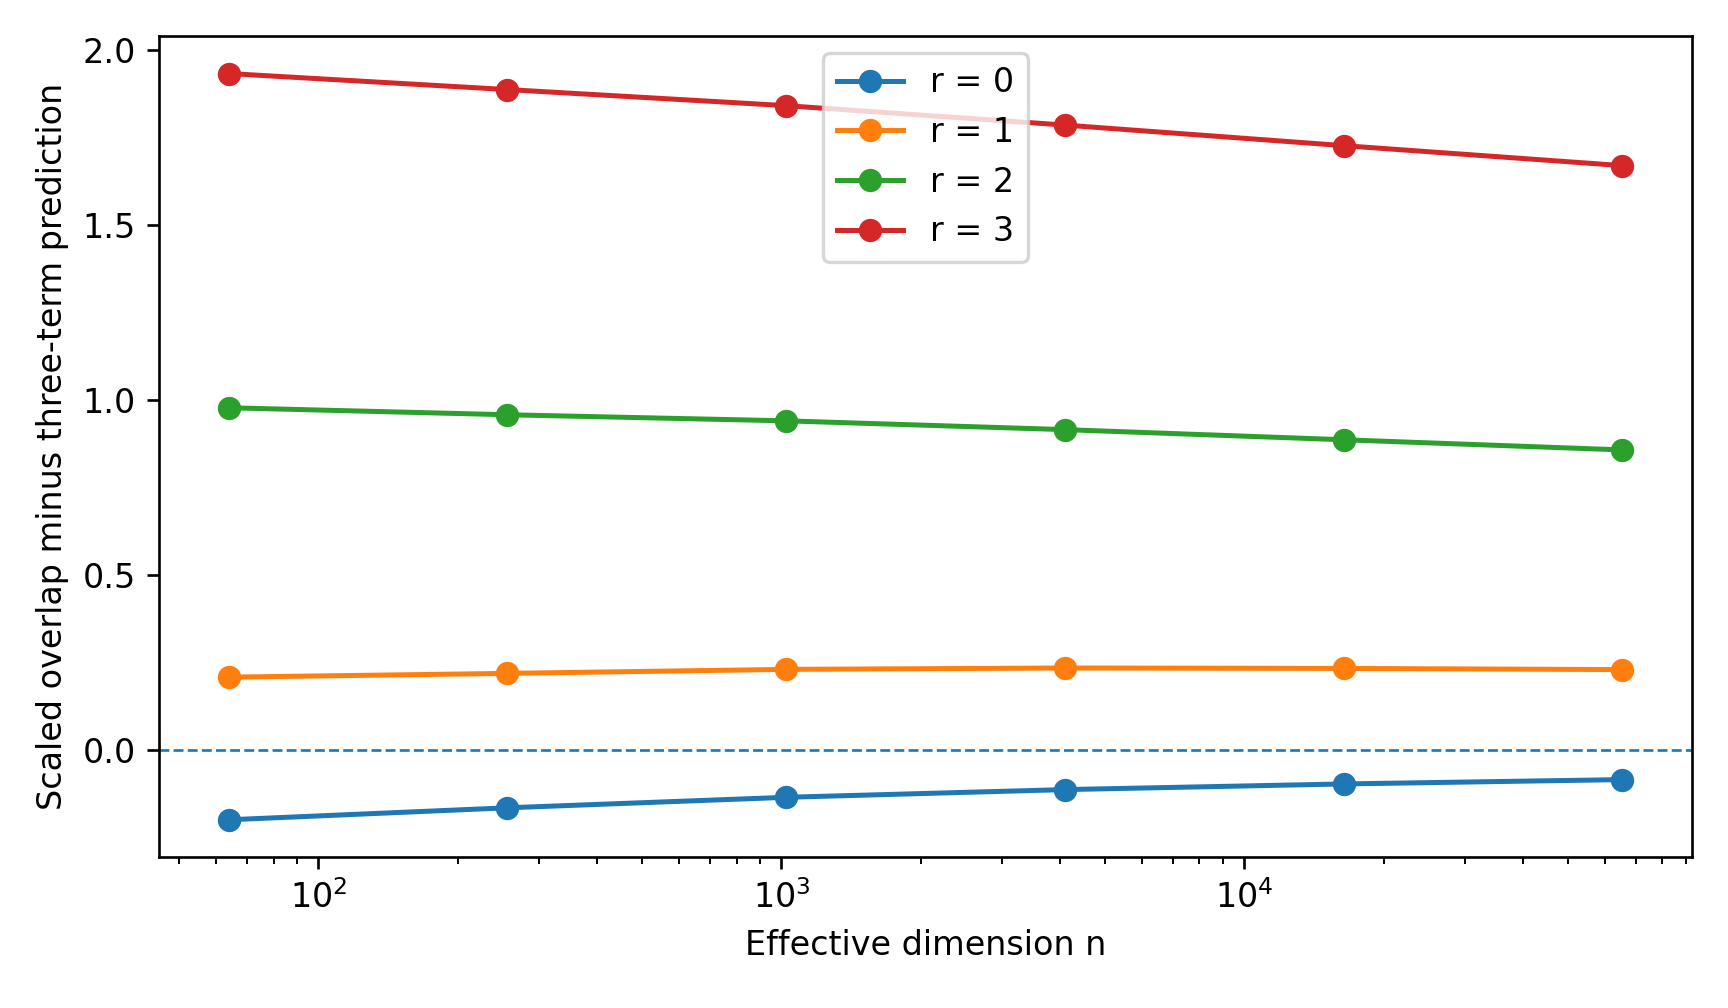
\includegraphics[width=.94\linewidth]{figures/overlap_residual.png}
\caption{Scaled overlap minus the three-term prediction in
\cref{thm:overlap}. The theorem is a fixed-$r$ asymptotic statement;
large visible residuals at these dimensions do not contradict it.
The explicit kernel reduction retains those corrections.}
\label{fig:residual}
\end{figure}

\begin{table}[H]
\centering\small
\begin{tabular}{rrrrrr}
\toprule
$n$ & $r$ & Scaled overlap & $J_r(c_n)$ & $\delta_r(c_n)$ & Difference\\
\midrule
1,024 & 0 & 5.735118 & 5.744889 & 0.125920 & -0.009771 \\
65,536 & 0 & 7.865122 & 7.865720 & 0.084530 & -0.000598 \\
1,024 & 1 & 7.578840 & 7.596856 & 0.259043 & -0.018016 \\
65,536 & 1 & 10.045763 & 10.046779 & 0.171746 & -0.001016 \\
1,024 & 2 & 9.074007 & 9.100505 & 0.471064 & -0.026498 \\
65,536 & 2 & 11.846601 & 11.848033 & 0.312294 & -0.001433 \\
1,024 & 3 & 10.354197 & 10.389753 & 0.767447 & -0.035556 \\
65,536 & 3 & 13.426689 & 13.428555 & 0.513576 & -0.001866 \\
\bottomrule
\end{tabular}

\caption{The fixed-kernel reduction is considerably more accurate at
finite $n$ than the three-term expansion. ``Difference'' is the scaled
overlap minus $J_r(c_n)$. The endpoint defect remains appreciable even
at $n=65536$, particularly for larger fixed $r$.}
\label{tab:reduction}
\end{table}

\begin{figure}[H]
\centering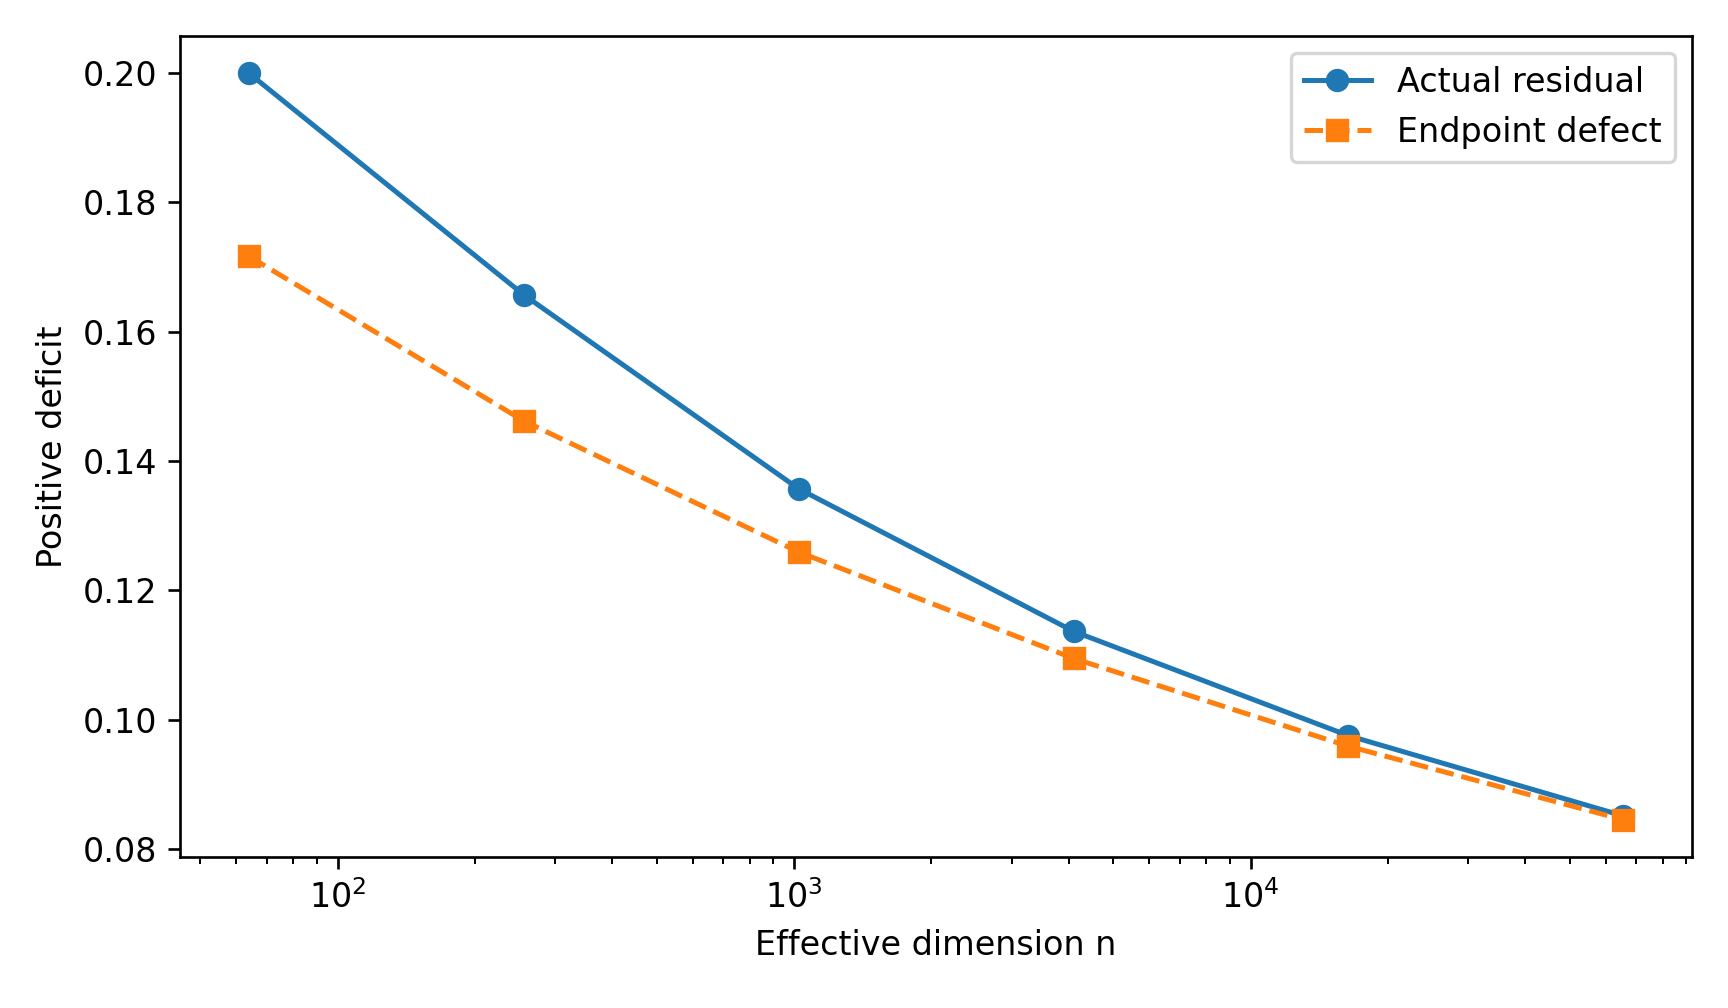
\includegraphics[width=.94\linewidth]{figures/endpoint_defect.png}
\caption{For $r=0$, the deficit from $\Lambda_n+\log K+1$ compared
with the boundary defect $\delta_0(c_n)$. Their difference is the bulk
local-density correction. This plot checks the structural identity;
it is not a numerical determination of the eventual logarithmic
exponent in \cref{thm:flatmain}.}
\label{fig:defect}
\end{figure}

\begin{table}[H]
\centering\small
\begin{tabular}{rrrr}
\toprule
$r$ & $h(H_r)$ & $h_{1/2}(H_r)$ & Normalization error\\
\midrule
0 & 1.14084719 & 1.48847380 & -8.79e-11 \\
1 & 1.60461229 & 1.86924365 & -7.28e-11 \\
2 & 1.85877132 & 2.09397602 & -2.08e-11 \\
3 & 2.02988383 & 2.25179053 & -1.72e-12 \\
\bottomrule
\end{tabular}

\caption{Boundary entropy constants for $q=1/2$, $\rho=1$.
The symbols $h(H_r)$ and $h_{1/2}(H_r)$ in the table denote
$\mathfrak h_1(h_r)$ and $\mathfrak h_{1/2}(h_r)$, respectively.
The last column is the numerical integral of the kernel minus one,
not an a priori error estimate.}
\label{tab:entropy}
\end{table}

\begin{figure}[H]
\centering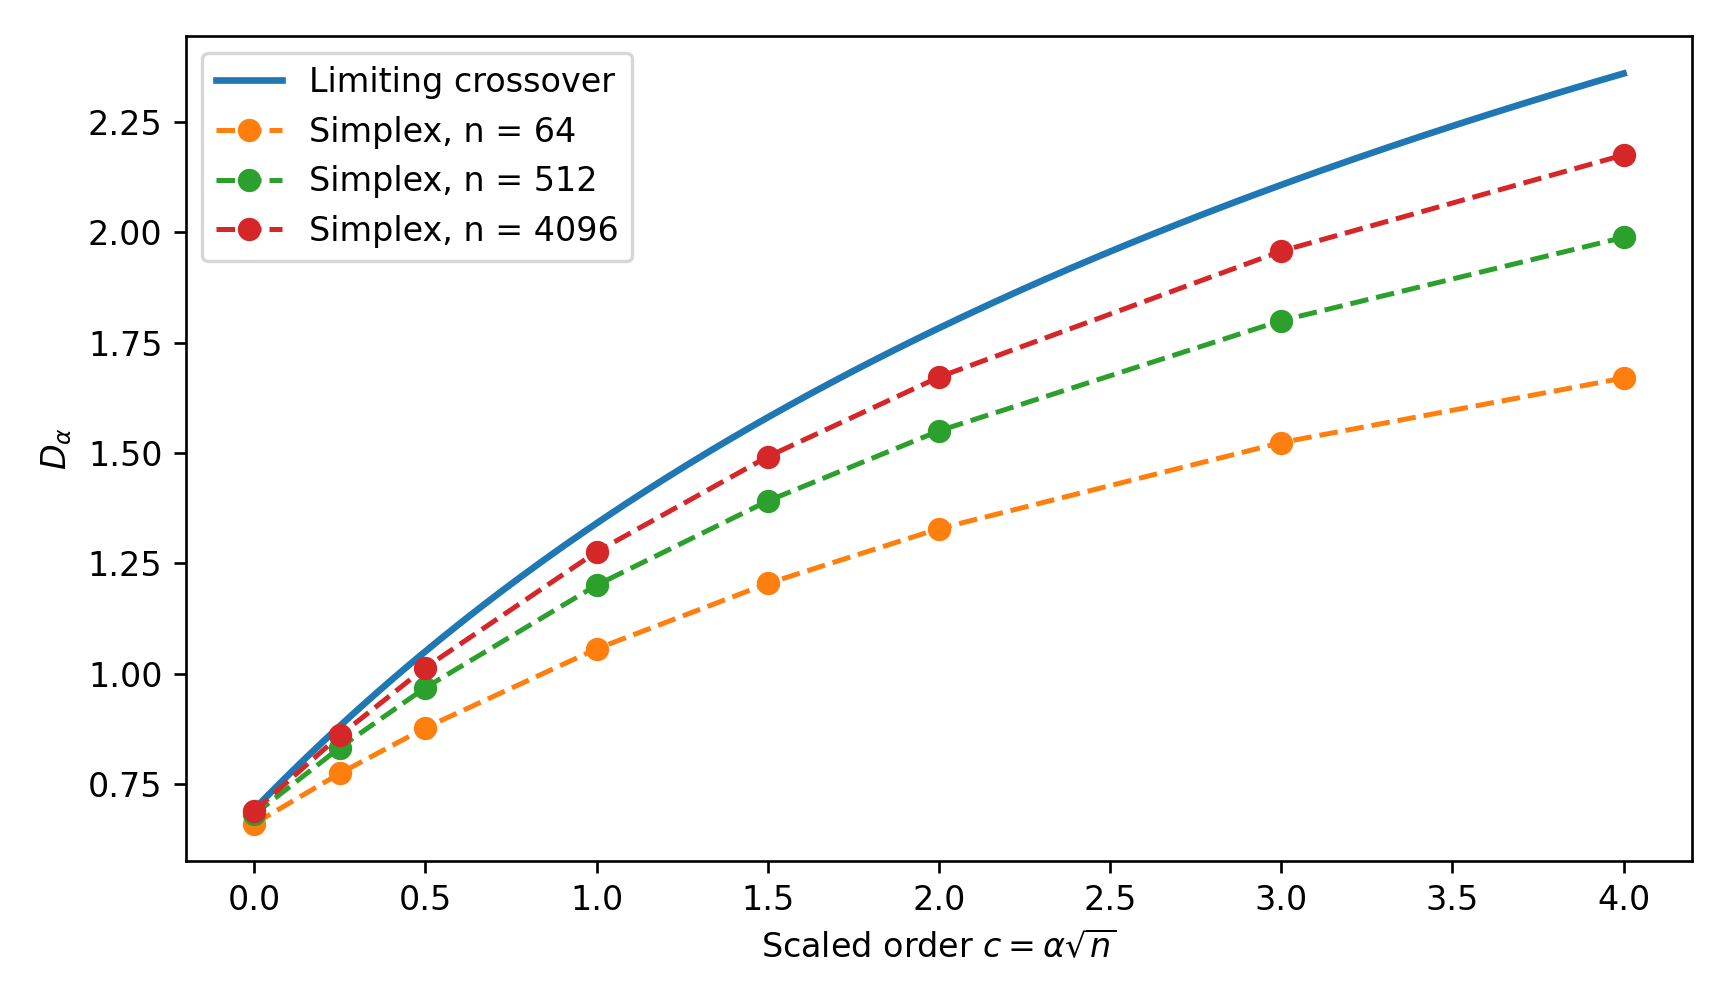
\includegraphics[width=.94\linewidth]{figures/renyi_crossover.png}
\caption{The universal order-zero transition, compared with
finite-simplex integrals at $r=0$. These are an independent benchmark,
not geometric-series observations. The finite-dimensional bias is
visible, especially for larger scaled order $c$.}
\label{fig:crossover}
\end{figure}

\subsection{How to reproduce the calculations}
Run \texttt{python code/verify.py} from the package directory.
The verification receipt is written to \path{data/verification.json}.
The script also writes exact algebra records,
CSV diagnostics, table fragments, and the figures. The delivered
numerical run used Python 3.13.5, NumPy 2.3.5, SciPy 1.17.0,
SymPy 1.14.0, and mpmath 1.3.0. The environment is recorded in the
receipt. The PDF can be rebuilt independently of the numerical
calculation with \texttt{latexmk -pdf article.tex}; the generated
figures and table fragments are already included.

\section{Further research questions and a development plan}
\label{sec:future}
The results settle the fixed-$r$, bounded-complement slice of the
repository's critical-complement question. They leave a structured set
of next problems. The statements in this section are questions and
proposed targets, not additional theorems.

\subsection{From fixed complements to growing complements}
\begin{question}[A uniform mesoscopic complement theory]
Let $r=r_n\to\infty$ while $r_n=o(n)$, and observe
$\{r_n+1,\ldots,n\}$. What uniform overlap and information formulas
interpolate between the non-Gaussian critical kernel and the
fixed-fraction Gaussian profile?
\end{question}
The early-cap cancellation remains exact whenever the deleted caps
exceed the constraint, but the gamma shape in $H_{r_n}$ now grows.
The polynomial degree, entropy, and clipping threshold all move.
The main obstruction is no longer discovering a kernel; it is
controlling the bulk density on the entire range where that kernel
is clipped. A useful first target is an explicit regime such as
$r_n(\log n)^2=o(n)$, followed by identification of the sharp
condition. That displayed regime is a suggested starting point,
not a proved sufficient condition here.
% ed. (2026-10-01): the logarithmic slice of this question is answered by a later package (batch 71).
\begin{ednotelater}
The logarithmic slice of this question is answered, for the overlap
only, by a later article, \emph{Second Order Critical Complements in
Fabius Conditioning}, filed as
\path{../Second_Order_Critical_Complements_Fabius_Conditioning/}
(batch~71 of the repository's \path{docs/incoming/}; unreviewed). Its
``early'' mask observes $\{r_n+1,\ldots,n\}$ (its ``early'' and ``late''
name the hidden coordinates), and its tilt is $\rho'q^{-(n+1)}$, so
$\rho=\rho'/q$ as in the note at the end of Section~1.1. Uniformly for
$c_0\log n\le r_n\le c_1\log n$, with $0<c_0<c_1$ fixed, it proves
\[
\frac{\OO_{n,r_n}}{c_n}=r_n(y_+-y_-)+[F]_{y_-}^{y_+}
 +\frac1{r_n}[B]_{y_-}^{y_+}
 +O\Bigl(\frac1{r_n^2}+\frac{r_n^3}{n}\Bigr),\qquad
F(y)=\frac{\log\E e^{(1-1/y)R_\rho}+1}{1-1/y},
\]
where $y_-<1<y_+$ solve $y-1-\log y=\log(n/r_n)/(2r_n)$ and $B$ is an
explicit coefficient built from the same moment generating function. The
leading term is the Lambert-$W$ crossover that
\path{../Critical_Complements_Sharp_Information_Loss/} (its Theorem~2.2)
proves for the other mask, which hides the last $r_n$ bulk coordinates.
By \eqref{eq:R}, $\E e^{R_\rho}=K$; so as $r_n/\log n=c\downarrow0$ the
constant $[F]_{y_-}^{y_+}$ tends to $\log K+1$, the constant of
\eqref{eq:mainoverlap} at $r=0$ (a consistency check outside the
theorem's range; the value $\log K=0.486134172\ldots$ of
\eqref{eq:dyadicconstants} was reproduced on filing as
$\log\E e^{R_\rho}$, to 30 digits). It also proves that for
$r_n/\log n\to c\in(0,\infty)$ the block observed here keeps eventually
strictly more overlap than the prefix $\{1,\ldots,n-r_n\}$, as it does
for fixed $r\ge1$ by \eqref{eq:mainoverlap} and that article's
Theorem~2.1, where the gap grows like $r\log\Lambda_n$. Thinner and
thicker growing complements ($r_n/\log n\to0$ or $\infty$), uniformity
as $c\downarrow0$ or $c\to\infty$, and the information formulas asked
for here remain open.
\end{ednotelater}

\begin{question}[The optimal finite-$n$ error]
Can the $O((\log n)^3/n)$ error in \eqref{eq:quantJ} be replaced by
an explicit signed expansion with a computable remainder, uniformly
over a compact set of phases?
\end{question}
The proof deliberately takes suprema over a logarithmic window.
Retaining the quadratic and cubic terms of the centered gamma
core and the exact low cumulants of the short boundary block should
give a more efficient expansion. Its coefficients would interact
with truncated moments of $\min(1,h_r/c_n)$, rather than only
ordinary moments. A rigorous answer must control the signed gamma
mixture or another positive representation without assuming a
formal expansion is uniformly integrable.

\subsection{Endpoint defects beyond their leading logarithm}
\begin{question}[A sharp asymptotic equivalent for the defect]
Determine $\delta_r(c_n)$ up to a multiplicative $1+o(1)$ error,
including any phase-sensitive corrections inherited from the
small-ball asymptotics of $T_\rho$.
\end{question}
We proved its logarithm only to leading square-root order.
A refined small-ball formula has to be inverted at the moving
level $h_r(w)=c_n$, and then integrated across the transition.
The integral need not equal the lower crossing to relative error
$o(1)$ without an additional steepness estimate. This is where the
repository's exact-phase scalar endpoint machinery could supply
more than the elementary bounds used in this article.

\begin{question}[Inverse reconstruction from critical information]
To what extent do the functions $r\mapsto\mathfrak h_\alpha(h_r)$,
the phase constant $K$, and the defects $\delta_r(z)$ determine the
underlying boundary law?
\end{question}
The upper-tail polynomials already recover successive ordinary
moments once $K$ is known. Since the boundary support is compact,
all moments determine its law. The more difficult question is how
much information is retained when only entropies or asymptotic
coefficients of a fixed observed block are available. A stability
result would be more useful than uniqueness alone.

\subsection{Information-order transitions and different constraints}
\begin{question}[Uniform matching of R\'enyi orders]
Find a single approximation valid from $\alpha=0$ through
$\alpha\sqrt n\to\infty$, and into fixed positive orders.
\end{question}
The limiting function in \eqref{eq:crossovermatch} matches the
formal small-order limit of the fixed-order formula. A proof must
control $h_r(w)^\alpha$ when its mass explores both the
$w=O(1)$ and $w=O(\sqrt n)$ regions. The first correction may
separate universal bulk terms from $r$- and phase-dependent terms.
Uniform treatment near order one would then connect this matching
to relative entropy without a removable-singularity loss.

\begin{question}[Several inequalities or a thin conditioning window]
What replaces the single gamma-slack kernel under two independent
linear constraints, a cone constraint, or conditioning on
$\mu_n-a_n\le t_nS_q\le\mu_n$?
\end{question}
For a fixed-width window the one-sided exponential slack must be
truncated. For several constraints the relevant local object is a
multivariate boundary law integrated over a feasible cone, and the
canonical normalizing density is matrix-valued. One should first
prove the analogue of \cref{thm:exact} in a concrete two-dimensional
example; simply replacing a scalar variance by a determinant does
not account for the cone geometry.

\subsection{Other coordinate laws and formal computation}
\begin{question}[Gamma universality and its failures]
Suppose the coordinate density behaves near zero like
$u^{\beta-1}\ell(u)$, with $\beta>0$. Under what hypotheses does the
critical kernel become a boundary tail plus a gamma variable of
shape $r\beta+1$?
\end{question}
A gamma limit for each strongly tilted lost coordinate is a natural
candidate. Unlike the uniform case, however, an eventually exact
cancellation of all early caps and density factors is generally
unavailable. Rates for the local density and for the approximation
of the early digits must be proved jointly. Slowly varying factors,
nonlog-concave densities, and atoms at zero may yield genuinely
different behavior.

\begin{question}[Formal verification and certified numerical kernels]
Can the moment-polynomial identities, exact kernel reduction, and
local gamma-core bounds be formalized as reusable Lean lemmas,
and can the accompanying numerical formulas be evaluated with
certified intervals?
\end{question}
A practical dependency order is: finite product tilting and pushforward
likelihoods; gamma convolution and polynomial tails; exact rational
moment recursion; the gamma-core local estimate; normalization and
clipped-density comparison; finally entropy and moving-order limits.
The finite algebra is a comparatively small first formalization target.
The analytic layer needs countable product probability spaces,
measure changes, convolution, and dominated-convergence infrastructure.
No uncompiled Lean skeleton is included as evidence of verification.

For certified computation, a positive boundary-convolution algorithm
with interval CDF bounds avoids alternating cancellation near the flat
endpoint. The bulk can then be bounded by interval versions of the
gamma-core decomposition. A final error budget must separately account
for tail truncation, discretization, quadrature, root location, and
rounding; the current refinement comparisons do not provide that budget.

\section{Conclusion and proof-status boundary}
The earlier variance-fraction theorem says that an almost complete
active block eventually separates from its tilted product marginal.
In the fixed critical-complement regime, the present results quantify
that separation and identify what survives below the Gaussian scale.
The missing early digits contribute a gamma shape, the infinite
geometric tail contributes a phase-dependent density, and clipping
that density determines the exact logarithmic overlap hierarchy.

At every fixed positive information order, a boundary differential
entropy supplies the finite correction to the diverging bulk term.
At order zero the support remains macroscopic, producing $\log2$
instead. The universal crossover makes the noncommutation of these
limits explicit. Finally, when no early digit is omitted, all
inverse-logarithmic upper-tail corrections disappear; the remaining
signed discrepancy directly reveals the flat Fabius endpoint.

The mathematical claims labelled as theorems and propositions have
proofs in this manuscript. They have not been externally refereed or
compiled in Lean. The numerical script verifies finite algebraic
identities and performs floating-point diagnostics only. The proposed
novelty is relative to the inspected repository question and the
reviewed references; neither an exhaustive priority search nor a
resolution of every formulation of the critical-complement problem
is claimed.

\appendix
\section{Repository provenance and inspection scope}
\label{app:provenance}
The repository tree was pinned at
\begin{center}\small\sha\end{center}
The baseline manuscript is located under
\begin{quote}\small\ttfamily\raggedright
Analysis/FabiusFunction/docs/\allowbreak
semi-formalized-research-frontiers/drafts/\allowbreak
representations/\allowbreak
Sharp\_Conditioning\_Laws\_Uniform\_Random\_Series/
\end{quote}
Its \texttt{article.tex} blob identifier is
\begin{center}\small\texttt{55945402782d507eb59dfd195514037ef41fb964}.
\end{center}
We inspected the baseline README and claim-status ledger, and the
source's explicit research questions, including \texttt{q:critical}
and \texttt{q:edgeworth}, at this pinned reference. We also inspected
its later proof/discussion sections for context. The full repository
was not rebuilt, nor were all archived manuscripts exhaustively
searched. GitHub code search may lag a branch tip, so absence from a
search result was not treated as proof of novelty.

The baseline's claim ledger explicitly excludes quantitative uniform
bounds near retained variance fraction one. Our error estimates are
for fixed $r$ and fixed geometric parameters, not the uniform
shrinking-complement-fraction bounds posed in its most general
question. This distinction is part of the theorem statements, not
merely an implementation limitation.

The external review used the primary arXiv records of the Fabius,
small-deviation, and R\'enyi references, together with the original
conditional-limit reference's bibliographic record. This was a
targeted relevance and attribution check, not an exhaustive
full-text literature survey. All analytic steps specific to the
new theorem package are supplied in the article.

\section{Package map}
\label{app:package}
\noindent
\texttt{article.tex} and \texttt{article.pdf} are the complete source and
compiled manuscript. The source inputs the generated table fragments
from \texttt{data/} and the three PNG figures in \texttt{figures/}.
\texttt{code/verify.py} reproduces the exact checks, diagnostics,
tables, and figures. \texttt{data/exact\_algebra.json} contains the
rational moments and tail polynomials; \texttt{data/verification.json}
records counts, numerical constants, and the executed environment.
\texttt{README.md}, \texttt{CLAIM\_STATUS.md},
\texttt{provenance.json}, and \texttt{validation.json} document the
scope and artifact checks. No font files are distributed.

\begin{thebibliography}{9}
\bibitem{repoSharp}
\repo{} repository.
\emph{Sharp Conditioning Laws for Uniform Random Series:
Variance thresholds, boundary phases, Brownian bridges, and rare-event
sampling}. Research manuscript dated September 28, 2026, with README
and claim-status ledger. Pinned reference and path are recorded in
Appendix~\ref{app:provenance}.
\url{https://github.com/VladimirReshetnikov/ProveIt}.

\bibitem{arias}
Juan Arias de Reyna.
\emph{An infinitely differentiable function with compact support:
Definition and properties}. English translation of the author's
1982 paper, arXiv:1702.05442, 2017.
\url{https://arxiv.org/abs/1702.05442}.

\bibitem{arithmetic}
Juan Arias de Reyna.
\emph{Arithmetic of the Fabius function}. arXiv:1702.06487v3, 2017.
\url{https://arxiv.org/abs/1702.06487}.

\bibitem{aurzada}
Frank Aurzada.
\emph{A short note on small deviations of sequences of i.i.d. random
variables with exponentially decreasing weights}.
Statistics \& Probability Letters \textbf{78} (2008), 2300--2307.
arXiv:0711.2576.
\url{https://arxiv.org/abs/0711.2576}.

\bibitem{df}
Persi Diaconis and David Freedman.
\emph{Conditional limit theorems for exponential families and finite
versions of de Finetti's theorem}.
Journal of Theoretical Probability \textbf{1} (1988), 381--410.
\url{https://doi.org/10.1007/BF01048727}.

\bibitem{renyi}
Tim van Erven and Peter Harremo\"es.
\emph{R\'enyi divergence and Kullback--Leibler divergence}.
IEEE Transactions on Information Theory \textbf{60} (2014), 3797--3820.
arXiv:1206.2459.
\url{https://arxiv.org/abs/1206.2459}.
\end{thebibliography}
\end{document}
